% Options for packages loaded elsewhere
\PassOptionsToPackage{unicode}{hyperref}
\PassOptionsToPackage{hyphens}{url}
%
\documentclass[
]{article}
\usepackage{lmodern}
\usepackage{amsmath}
\usepackage{ifxetex,ifluatex}
\ifnum 0\ifxetex 1\fi\ifluatex 1\fi=0 % if pdftex
  \usepackage[T1]{fontenc}
  \usepackage[utf8]{inputenc}
  \usepackage{textcomp} % provide euro and other symbols
  \usepackage{amssymb}
\else % if luatex or xetex
  \usepackage{unicode-math}
  \defaultfontfeatures{Scale=MatchLowercase}
  \defaultfontfeatures[\rmfamily]{Ligatures=TeX,Scale=1}
\fi
% Use upquote if available, for straight quotes in verbatim environments
\IfFileExists{upquote.sty}{\usepackage{upquote}}{}
\IfFileExists{microtype.sty}{% use microtype if available
  \usepackage[]{microtype}
  \UseMicrotypeSet[protrusion]{basicmath} % disable protrusion for tt fonts
}{}
\makeatletter
\@ifundefined{KOMAClassName}{% if non-KOMA class
  \IfFileExists{parskip.sty}{%
    \usepackage{parskip}
  }{% else
    \setlength{\parindent}{0pt}
    \setlength{\parskip}{6pt plus 2pt minus 1pt}}
}{% if KOMA class
  \KOMAoptions{parskip=half}}
\makeatother
\usepackage{xcolor}
\IfFileExists{xurl.sty}{\usepackage{xurl}}{} % add URL line breaks if available
\IfFileExists{bookmark.sty}{\usepackage{bookmark}}{\usepackage{hyperref}}
\hypersetup{
  pdftitle={Final\_Proj},
  pdfauthor={Khoa Nguyen},
  hidelinks,
  pdfcreator={LaTeX via pandoc}}
\urlstyle{same} % disable monospaced font for URLs
\usepackage[margin=1in]{geometry}
\usepackage{color}
\usepackage{fancyvrb}
\newcommand{\VerbBar}{|}
\newcommand{\VERB}{\Verb[commandchars=\\\{\}]}
\DefineVerbatimEnvironment{Highlighting}{Verbatim}{commandchars=\\\{\}}
% Add ',fontsize=\small' for more characters per line
\usepackage{framed}
\definecolor{shadecolor}{RGB}{248,248,248}
\newenvironment{Shaded}{\begin{snugshade}}{\end{snugshade}}
\newcommand{\AlertTok}[1]{\textcolor[rgb]{0.94,0.16,0.16}{#1}}
\newcommand{\AnnotationTok}[1]{\textcolor[rgb]{0.56,0.35,0.01}{\textbf{\textit{#1}}}}
\newcommand{\AttributeTok}[1]{\textcolor[rgb]{0.77,0.63,0.00}{#1}}
\newcommand{\BaseNTok}[1]{\textcolor[rgb]{0.00,0.00,0.81}{#1}}
\newcommand{\BuiltInTok}[1]{#1}
\newcommand{\CharTok}[1]{\textcolor[rgb]{0.31,0.60,0.02}{#1}}
\newcommand{\CommentTok}[1]{\textcolor[rgb]{0.56,0.35,0.01}{\textit{#1}}}
\newcommand{\CommentVarTok}[1]{\textcolor[rgb]{0.56,0.35,0.01}{\textbf{\textit{#1}}}}
\newcommand{\ConstantTok}[1]{\textcolor[rgb]{0.00,0.00,0.00}{#1}}
\newcommand{\ControlFlowTok}[1]{\textcolor[rgb]{0.13,0.29,0.53}{\textbf{#1}}}
\newcommand{\DataTypeTok}[1]{\textcolor[rgb]{0.13,0.29,0.53}{#1}}
\newcommand{\DecValTok}[1]{\textcolor[rgb]{0.00,0.00,0.81}{#1}}
\newcommand{\DocumentationTok}[1]{\textcolor[rgb]{0.56,0.35,0.01}{\textbf{\textit{#1}}}}
\newcommand{\ErrorTok}[1]{\textcolor[rgb]{0.64,0.00,0.00}{\textbf{#1}}}
\newcommand{\ExtensionTok}[1]{#1}
\newcommand{\FloatTok}[1]{\textcolor[rgb]{0.00,0.00,0.81}{#1}}
\newcommand{\FunctionTok}[1]{\textcolor[rgb]{0.00,0.00,0.00}{#1}}
\newcommand{\ImportTok}[1]{#1}
\newcommand{\InformationTok}[1]{\textcolor[rgb]{0.56,0.35,0.01}{\textbf{\textit{#1}}}}
\newcommand{\KeywordTok}[1]{\textcolor[rgb]{0.13,0.29,0.53}{\textbf{#1}}}
\newcommand{\NormalTok}[1]{#1}
\newcommand{\OperatorTok}[1]{\textcolor[rgb]{0.81,0.36,0.00}{\textbf{#1}}}
\newcommand{\OtherTok}[1]{\textcolor[rgb]{0.56,0.35,0.01}{#1}}
\newcommand{\PreprocessorTok}[1]{\textcolor[rgb]{0.56,0.35,0.01}{\textit{#1}}}
\newcommand{\RegionMarkerTok}[1]{#1}
\newcommand{\SpecialCharTok}[1]{\textcolor[rgb]{0.00,0.00,0.00}{#1}}
\newcommand{\SpecialStringTok}[1]{\textcolor[rgb]{0.31,0.60,0.02}{#1}}
\newcommand{\StringTok}[1]{\textcolor[rgb]{0.31,0.60,0.02}{#1}}
\newcommand{\VariableTok}[1]{\textcolor[rgb]{0.00,0.00,0.00}{#1}}
\newcommand{\VerbatimStringTok}[1]{\textcolor[rgb]{0.31,0.60,0.02}{#1}}
\newcommand{\WarningTok}[1]{\textcolor[rgb]{0.56,0.35,0.01}{\textbf{\textit{#1}}}}
\usepackage{graphicx}
\makeatletter
\def\maxwidth{\ifdim\Gin@nat@width>\linewidth\linewidth\else\Gin@nat@width\fi}
\def\maxheight{\ifdim\Gin@nat@height>\textheight\textheight\else\Gin@nat@height\fi}
\makeatother
% Scale images if necessary, so that they will not overflow the page
% margins by default, and it is still possible to overwrite the defaults
% using explicit options in \includegraphics[width, height, ...]{}
\setkeys{Gin}{width=\maxwidth,height=\maxheight,keepaspectratio}
% Set default figure placement to htbp
\makeatletter
\def\fps@figure{htbp}
\makeatother
\setlength{\emergencystretch}{3em} % prevent overfull lines
\providecommand{\tightlist}{%
  \setlength{\itemsep}{0pt}\setlength{\parskip}{0pt}}
\setcounter{secnumdepth}{-\maxdimen} % remove section numbering
\ifluatex
  \usepackage{selnolig}  % disable illegal ligatures
\fi

\title{Final\_Proj}
\author{Khoa Nguyen}
\date{3/9/2021}

\begin{document}
\maketitle

\begin{Shaded}
\begin{Highlighting}[]
\ControlFlowTok{if}\NormalTok{ ( }\SpecialCharTok{!}\FunctionTok{dir.exists}\NormalTok{( here}\SpecialCharTok{::}\FunctionTok{here}\NormalTok{(}\StringTok{"Final\_project"}\NormalTok{, }\StringTok{"data\_raw"}\NormalTok{) ) ) \{}
  \FunctionTok{dir.create}\NormalTok{( here}\SpecialCharTok{::}\FunctionTok{here}\NormalTok{(}\StringTok{"Final\_project"}\NormalTok{, }\StringTok{"data\_raw"}\NormalTok{, }\StringTok{"output"}\NormalTok{, }\StringTok{".R"}\NormalTok{), }\AttributeTok{recursive =} \ConstantTok{TRUE}\NormalTok{ )}
\NormalTok{\}}
\end{Highlighting}
\end{Shaded}

\hypertarget{divorce-rate-trend-and-marriage-rate-trend-comparison.}{%
\section{Divorce rate trend and Marriage Rate Trend
Comparison.}\label{divorce-rate-trend-and-marriage-rate-trend-comparison.}}

\hypertarget{research-questions.}{%
\subsection{Research Questions.}\label{research-questions.}}

\begin{quote}
Is the differences between the marriage trend and dicorve trend
throughout the years significant enough for us to reconsider what is the
criteria for a committed marriage? This is also a follow-up to the
original study.
\end{quote}

\begin{Shaded}
\begin{Highlighting}[]
\NormalTok{url }\OtherTok{\textless{}{-}} \StringTok{"https://raw.githubusercontent.com/fivethirtyeight/data/master/marriage/divorce.csv"}
\NormalTok{bothsexes }\OtherTok{\textless{}{-}} \StringTok{"https://raw.githubusercontent.com/fivethirtyeight/data/master/marriage/both\_sexes.csv"}
\NormalTok{men }\OtherTok{\textless{}{-}} \StringTok{"https://raw.githubusercontent.com/fivethirtyeight/data/master/marriage/men.csv"}
\NormalTok{women }\OtherTok{\textless{}{-}}  \StringTok{"https://raw.githubusercontent.com/fivethirtyeight/data/master/marriage/women.csv"}
\end{Highlighting}
\end{Shaded}

\begin{Shaded}
\begin{Highlighting}[]
\NormalTok{Major\_data }\OtherTok{\textless{}{-}} \FunctionTok{read.csv}\NormalTok{(url,}
                       \AttributeTok{na =} \FunctionTok{c}\NormalTok{(}\StringTok{"NA"}\NormalTok{, }\StringTok{" "}\NormalTok{, }\StringTok{"{-}999"}\NormalTok{))}
\NormalTok{both\_gender }\OtherTok{\textless{}{-}}  \FunctionTok{read.csv}\NormalTok{(bothsexes,}
                       \AttributeTok{na =} \FunctionTok{c}\NormalTok{(}\StringTok{"NA"}\NormalTok{, }\StringTok{" "}\NormalTok{, }\StringTok{"{-}999"}\NormalTok{))}
\NormalTok{men\_data }\OtherTok{\textless{}{-}}  \FunctionTok{read.csv}\NormalTok{(men,}
                       \AttributeTok{na =} \FunctionTok{c}\NormalTok{(}\StringTok{"NA"}\NormalTok{, }\StringTok{" "}\NormalTok{, }\StringTok{"{-}999"}\NormalTok{))}
\NormalTok{women\_data }\OtherTok{\textless{}{-}}  \FunctionTok{read.csv}\NormalTok{(women,}
                       \AttributeTok{na =} \FunctionTok{c}\NormalTok{(}\StringTok{"NA"}\NormalTok{, }\StringTok{" "}\NormalTok{, }\StringTok{"{-}999"}\NormalTok{))}
\end{Highlighting}
\end{Shaded}

\begin{Shaded}
\begin{Highlighting}[]
\FunctionTok{write.csv}\NormalTok{(Major\_data,}
\NormalTok{          here}\SpecialCharTok{::}\FunctionTok{here}\NormalTok{(}\StringTok{"Final\_project"}\NormalTok{, }\StringTok{"data\_raw"}\NormalTok{, }\StringTok{"Major\_data.csv"}\NormalTok{))}
\FunctionTok{write.csv}\NormalTok{(both\_gender,}
\NormalTok{          here}\SpecialCharTok{::}\FunctionTok{here}\NormalTok{(}\StringTok{"Final\_project"}\NormalTok{, }\StringTok{"data\_raw"}\NormalTok{, }\StringTok{"Both\_gender.csv"}\NormalTok{))}
\FunctionTok{write.csv}\NormalTok{(men\_data,}
\NormalTok{          here}\SpecialCharTok{::}\FunctionTok{here}\NormalTok{(}\StringTok{"Final\_project"}\NormalTok{, }\StringTok{"data\_raw"}\NormalTok{, }\StringTok{"Men\_data.csv"}\NormalTok{))}
\FunctionTok{write.csv}\NormalTok{(women\_data,}
\NormalTok{          here}\SpecialCharTok{::}\FunctionTok{here}\NormalTok{(}\StringTok{"Final\_project"}\NormalTok{, }\StringTok{"data\_raw"}\NormalTok{, }\StringTok{"Women\_data.csv"}\NormalTok{))}
\end{Highlighting}
\end{Shaded}

\begin{Shaded}
\begin{Highlighting}[]
\FunctionTok{read.csv}\NormalTok{(}
\NormalTok{  here}\SpecialCharTok{::}\FunctionTok{here}\NormalTok{(}\StringTok{"Final\_Project"}\NormalTok{, }\StringTok{"data\_raw"}\NormalTok{, }\StringTok{"Major\_data.csv"}\NormalTok{))}
\end{Highlighting}
\end{Shaded}

\begin{verbatim}
##    X.1  X year       date   all_3544    HS_3544    SC_3544   BAp_3544
## 1    1  1 1960 1960-01-01 0.03444454 0.03488887 0.03366938 0.02751277
## 2    2  2 1970 1970-01-01 0.04925600 0.04999984 0.04870549 0.04125945
## 3    3  3 1980 1980-01-01 0.10600503 0.10415128 0.11269947 0.09777208
## 4    4  4 1990 1990-01-01 0.15080495 0.15938095 0.16967005 0.11495533
## 5    5  5 2000 2000-01-01 0.15684099 0.17544616 0.17380324 0.10561772
## 6    6  6 2001 2001-01-01 0.15730639 0.17411604 0.17816906 0.10703886
## 7    7  7 2002 2002-01-01 0.15650825 0.17476931 0.17929419 0.10344219
## 8    8  8 2003 2003-01-01 0.15384351 0.17254483 0.17697536 0.10254990
## 9    9  9 2004 2004-01-01 0.15484096 0.17756455 0.17707955 0.10033665
## 10  10 10 2005 2005-01-01 0.15291994 0.17516353 0.17674265 0.09948066
## 11  11 11 2006 2006-01-01 0.16188986 0.18943673 0.18412098 0.10383550
## 12  12 12 2007 2007-01-01 0.16046887 0.18721641 0.18496086 0.10392942
## 13  13 13 2008 2008-01-01 0.16115876 0.18837663 0.18944998 0.10201919
## 14  14 14 2009 2009-01-01 0.16049309 0.18698758 0.19013626 0.10194261
## 15  15 15 2010 2010-01-01 0.16365109 0.18989580 0.19726945 0.10306385
## 16  16 16 2011 2011-01-01 0.16630283 0.19239892 0.20045883 0.10776053
## 17  17 17 2012 2012-01-01 0.16548645 0.19020633 0.20317649 0.10740666
##      BAo_3544    GD_3544  poor_3544   mid_3544  rich_3544   all_4554    HS_4554
## 1  0.02751277         NA 0.07195136 0.02122530 0.02256233 0.03965056 0.04007142
## 2  0.04125945         NA 0.11373582 0.03030104 0.02192707 0.05062562 0.05056576
## 3  0.09777208         NA 0.24164705 0.07367154 0.03501521 0.08818511 0.08566351
## 4  0.11853432 0.10914537 0.32694839 0.11190969 0.04972527 0.14572572 0.14077914
## 5  0.11053969 0.09590347 0.34308859 0.11658371 0.04939497 0.17958060 0.18477676
## 6  0.11186064 0.09719692 0.34283554 0.12278063 0.04057431 0.18265130 0.19023658
## 7  0.10968956 0.09076255 0.34108826 0.11992642 0.03879621 0.18065043 0.19209040
## 8  0.11068292 0.08638486 0.33310488 0.12104747 0.03926215 0.18469755 0.19489113
## 9  0.10598952 0.08911388 0.33432769 0.12193014 0.03679592 0.18411122 0.19373941
## 10 0.10711496 0.08499205 0.32907368 0.12240404 0.03707052 0.18432461 0.19721310
## 11 0.11085833 0.09050269 0.33716665 0.12610861 0.05789479 0.19614988 0.21070770
## 12 0.11188233 0.08905043 0.33523025 0.12220858 0.05816887 0.19496022 0.21274409
## 13 0.11115289 0.08519438 0.33373946 0.12471831 0.06033570 0.19763060 0.21682432
## 14 0.11183907 0.08439307 0.33001493 0.12468418 0.05997526 0.19764930 0.21797512
## 15 0.11163171 0.08816742 0.32872407 0.13381959 0.05776135 0.20350999 0.22431650
## 16 0.11728367 0.09188349 0.32954144 0.13836406 0.05881448 0.20329632 0.22563247
## 17 0.11529188 0.09431368 0.33156037 0.13307736 0.05635499 0.20738890 0.22866852
##       SC_4554   BAp_4554   BAo_4554   GD_4554  poor_4554   mid_4554  rich_4554
## 1  0.03870331 0.03188568 0.03188568        NA 0.07537252 0.02933657 0.02350489
## 2  0.05147270 0.04831053 0.04831053        NA 0.11249624 0.03386947 0.02123280
## 3  0.09500947 0.09103488 0.09103488        NA 0.19867321 0.06300866 0.02791567
## 4  0.16633103 0.13436974 0.13566093 0.1327413 0.30661378 0.11498064 0.04577501
## 5  0.20110350 0.14904161 0.15369313 0.1425498 0.38213542 0.14224209 0.05152510
## 6  0.20573707 0.14863163 0.15326921 0.1417453 0.39003850 0.14651347 0.04522236
## 7  0.19804840 0.14643862 0.15288797 0.1367771 0.38379508 0.14624231 0.04608881
## 8  0.20679189 0.14734955 0.15122316 0.1414393 0.39131512 0.15124003 0.04269424
## 9  0.20831171 0.14563041 0.15184099 0.1357963 0.39119899 0.15075508 0.04106048
## 10 0.20527615 0.14348225 0.14739462 0.1373049 0.38939432 0.15080202 0.04277300
## 11 0.21940146 0.15039808 0.15688045 0.1397258 0.40197026 0.15917424 0.06352994
## 12 0.21656401 0.14659658 0.15319831 0.1355411 0.40641894 0.15482069 0.06371342
## 13 0.21963499 0.14663108 0.15138763 0.1385107 0.40912531 0.15600069 0.06670997
## 14 0.21947344 0.14445703 0.14993037 0.1351115 0.40676466 0.15796943 0.06757658
## 15 0.22446156 0.15059022 0.15816419 0.1372541 0.40980069 0.16715608 0.06969512
## 16 0.22444827 0.14875082 0.15538913 0.1370357 0.40742403 0.16900667 0.06762650
## 17 0.23181683 0.15247471 0.16008278 0.1393165 0.41006916 0.17446516 0.07038130
\end{verbatim}

\begin{Shaded}
\begin{Highlighting}[]
\FunctionTok{read.csv}\NormalTok{(}
\NormalTok{  here}\SpecialCharTok{::}\FunctionTok{here}\NormalTok{(}\StringTok{"Final\_Project"}\NormalTok{, }\StringTok{"data\_raw"}\NormalTok{, }\StringTok{"Both\_gender.csv"}\NormalTok{))}
\end{Highlighting}
\end{Shaded}

\begin{verbatim}
##    X.1  X year       date  all_2534   HS_2534   SC_2534  BAp_2534  BAo_2534
## 1    1  1 1960 1960-01-01 0.1233145 0.1095332 0.1522818 0.2389952 0.2389952
## 2    2  2 1970 1970-01-01 0.1269715 0.1094000 0.1495096 0.2187031 0.2187031
## 3    3  3 1980 1980-01-01 0.1991767 0.1617313 0.2236916 0.2881646 0.2881646
## 4    4  4 1990 1990-01-01 0.2968306 0.2777491 0.2780912 0.3612968 0.3656655
## 5    5  5 2000 2000-01-01 0.3450087 0.3316545 0.3249205 0.3874906 0.3939579
## 6    6  6 2001 2001-01-01 0.3527767 0.3446069 0.3341101 0.3835686 0.3925148
## 7    7  7 2002 2002-01-01 0.3535249 0.3490367 0.3361595 0.3774328 0.3870840
## 8    8  8 2003 2003-01-01 0.3620345 0.3581877 0.3418930 0.3873806 0.4000039
## 9    9  9 2004 2004-01-01 0.3673247 0.3708102 0.3450748 0.3847357 0.3976124
## 10  10 10 2005 2005-01-01 0.3793451 0.3870680 0.3596663 0.3886096 0.4029116
## 11  11 11 2006 2006-01-01 0.4147656 0.4312162 0.3912177 0.4147960 0.4298668
## 12  12 12 2007 2007-01-01 0.4269222 0.4441386 0.4084929 0.4209586 0.4389750
## 13  13 13 2008 2008-01-01 0.4394414 0.4599162 0.4235094 0.4297510 0.4473568
## 14  14 14 2009 2009-01-01 0.4625638 0.4845018 0.4469940 0.4518141 0.4743768
## 15  15 15 2010 2010-01-01 0.4697332 0.4942221 0.4544084 0.4561005 0.4768130
## 16  16 16 2011 2011-01-01 0.4833335 0.5115703 0.4685570 0.4658246 0.4901602
## 17  17 17 2012 2012-01-01 0.4943453 0.5235212 0.4799344 0.4766357 0.5022621
##      GD_2534 White_2534 Black_2534 Hisp_2534   NE_2534   MA_2534 Midwest_2534
## 1         NA  0.1164848  0.1621855 0.1393736 0.1504184 0.1628934    0.1121467
## 2         NA  0.1179043  0.1855163 0.1298769 0.1517231 0.1640680    0.1153741
## 3         NA  0.1824126  0.3137500 0.1885440 0.2414327 0.2505925    0.1828339
## 4  0.3474505  0.2639256  0.4838556 0.2962372 0.3500384 0.3623321    0.2755046
## 5  0.3691740  0.3127149  0.5144994 0.3180681 0.4091852 0.4175565    0.3308022
## 6  0.3590304  0.3183506  0.5437985 0.3321214 0.4200581 0.4294281    0.3344332
## 7  0.3512848  0.3196691  0.5403976 0.3312613 0.4078044 0.4290529    0.3397041
## 8  0.3538130  0.3256812  0.5568954 0.3417513 0.4311918 0.4479922    0.3475709
## 9  0.3517729  0.3306283  0.5724015 0.3485789 0.4490854 0.4494016    0.3523802
## 10 0.3514251  0.3438759  0.5751731 0.3589544 0.4509719 0.4638508    0.3624805
## 11 0.3757228  0.3753122  0.6207795 0.3953588 0.4814884 0.4975251    0.3941999
## 12 0.3752763  0.3867121  0.6355313 0.4096196 0.4914396 0.5061395    0.4074371
## 13 0.3849744  0.3982802  0.6431092 0.4286496 0.5095196 0.5210837    0.4191507
## 14 0.3956936  0.4222356  0.6588438 0.4528061 0.5289023 0.5446246    0.4506093
## 15 0.4058705  0.4304896  0.6657126 0.4564257 0.5450851 0.5491727    0.4511969
## 16 0.4071756  0.4414346  0.6807420 0.4766545 0.5413288 0.5625737    0.4655502
## 17 0.4164583  0.4539900  0.6847088 0.4874031 0.5643478 0.5754134    0.4720884
##    South_2534 Mountain_2534 Pacific_2534 poor_2534   mid_2534 rich_2534
## 1   0.1090562    0.09152117    0.1198758 0.1371597 0.07514929 0.2066776
## 2   0.1126220    0.10293602    0.1374964 0.1717202 0.08159207 0.1724093
## 3   0.1688435    0.17434230    0.2334279 0.3100591 0.14825303 0.1851082
## 4   0.2639794    0.25264326    0.3319579 0.4199108 0.24320008 0.2783226
## 5   0.3099712    0.30621032    0.3753061 0.5033676 0.30202036 0.2717386
## 6   0.3182688    0.30980779    0.3844799 0.5178771 0.31716118 0.2532041
## 7   0.3230276    0.29686569    0.3836922 0.5174252 0.31824041 0.2534724
## 8   0.3250139    0.31071886    0.3946902 0.5297279 0.32823175 0.2516064
## 9   0.3341527    0.31078861    0.3972153 0.5367582 0.33561274 0.2522545
## 10  0.3473821    0.34127770    0.4038807 0.5519224 0.34766829 0.2620452
## 11  0.3847213    0.37115592    0.4464473 0.5730500 0.37075821 0.3442543
## 12  0.4001335    0.37737599    0.4572573 0.5904736 0.38129486 0.3543571
## 13  0.4082158    0.40015715    0.4723882 0.6053676 0.39423085 0.3626483
## 14  0.4273097    0.41776053    0.4956330 0.6213246 0.42399221 0.3775050
## 15  0.4434588    0.41018505    0.4968328 0.6301818 0.43190949 0.3846912
## 16  0.4584298    0.43050717    0.5078316 0.6430845 0.44452945 0.4007966
## 17  0.4649634    0.44282191    0.5288999 0.6531721 0.45612887 0.4106040
##      all_3544    HS_3544    SC_3544  BAp_3544  BAo_3544   GD_3544 White_3544
## 1  0.07058157 0.06860309 0.06663695 0.1326265 0.1326265        NA 0.06825586
## 2  0.06732520 0.06511964 0.06271724 0.1116899 0.1116899        NA 0.06250372
## 3  0.06883378 0.06429102 0.06531333 0.1056102 0.1056102        NA 0.05966739
## 4  0.11191800 0.11210043 0.09699372 0.1285172 0.1258567 0.1328018 0.09611312
## 5  0.15605881 0.16993703 0.13800404 0.1541238 0.1536299 0.1550970 0.13207032
## 6  0.15642529 0.16870156 0.13986044 0.1548151 0.1524923 0.1595169 0.13287455
## 7  0.15967630 0.16963608 0.14551591 0.1592764 0.1598992 0.1580095 0.13429516
## 8  0.16089927 0.17417009 0.14725088 0.1554106 0.1551795 0.1558697 0.13547343
## 9  0.16515941 0.18235854 0.14932870 0.1563267 0.1573123 0.1543631 0.13836500
## 10 0.16859543 0.18697637 0.15489782 0.1563589 0.1578731 0.1534703 0.14393044
## 11 0.19023319 0.22050747 0.16879323 0.1678529 0.1703584 0.1630544 0.15928999
## 12 0.19350017 0.22589739 0.17468243 0.1668970 0.1704744 0.1601205 0.16121407
## 13 0.19841872 0.23530549 0.18052867 0.1690407 0.1709024 0.1655896 0.16386453
## 14 0.20303760 0.24681017 0.18553105 0.1650282 0.1673079 0.1609548 0.16633994
## 15 0.20717662 0.25251765 0.19103915 0.1668872 0.1712057 0.1592707 0.16749425
## 16 0.21223063 0.26267964 0.19665025 0.1669555 0.1734778 0.1558495 0.17118001
## 17 0.21601743 0.26875607 0.20471722 0.1667594 0.1737169 0.1549444 0.17471037
##    Black_3544  Hisp_3544    NE_3544    MA_3544 Midwest_3544 South_3544
## 1  0.08836728 0.07307651 0.09194322 0.09347468   0.06863360 0.06026353
## 2  0.10290904 0.07070500 0.08570110 0.09040725   0.06156272 0.05966057
## 3  0.13140081 0.08110790 0.07997323 0.09744428   0.06070641 0.05914089
## 4  0.22010298 0.12194206 0.12785915 0.14354989   0.10157576 0.09637035
## 5  0.30239381 0.15469520 0.17327422 0.18819256   0.14539201 0.14230600
## 6  0.30857796 0.14953050 0.16653497 0.18315109   0.14794407 0.14312592
## 7  0.30969793 0.16445917 0.17898838 0.19382928   0.14770720 0.14461094
## 8  0.32264197 0.15220492 0.17519576 0.19448544   0.14939285 0.14936826
## 9  0.31890557 0.16955859 0.18414649 0.19578831   0.15015105 0.15413926
## 10 0.32319204 0.16559780 0.18871570 0.20219385   0.15405839 0.15472515
## 11 0.36554962 0.18732624 0.21054281 0.22890075   0.17759199 0.17503217
## 12 0.36562848 0.19918875 0.21241883 0.22687429   0.18021324 0.17931002
## 13 0.37545234 0.20685314 0.20630379 0.23814693   0.18293040 0.18091848
## 14 0.38737104 0.21543700 0.21295003 0.24450515   0.18692975 0.18754509
## 15 0.39011860 0.22186685 0.22056743 0.24625241   0.19219061 0.19384278
## 16 0.39898340 0.22889257 0.22055699 0.25116645   0.19866122 0.20062204
## 17 0.40443495 0.23339748 0.22781766 0.25783642   0.20166514 0.20386508
##    Mountain_3544 Pacific_3544 poor_3544   mid_3544  rich_3544   all_4554
## 1     0.04739747   0.05822486 0.1019749 0.04717272 0.08553870 0.07254649
## 2     0.04651163   0.06347796 0.1117548 0.04566838 0.06499159 0.05968794
## 3     0.04880077   0.07552538 0.1291426 0.05050321 0.04445951 0.05250871
## 4     0.09189904   0.13134638 0.2012208 0.09024739 0.06573916 0.05947824
## 5     0.13584194   0.17480047 0.2813137 0.12815751 0.08622046 0.08804394
## 6     0.13943820   0.17694864 0.2919112 0.13267625 0.06803283 0.08823342
## 7     0.13424491   0.18279935 0.2904300 0.13723226 0.07153439 0.09284694
## 8     0.12944378   0.17966719 0.2967686 0.13791654 0.06949005 0.09697308
## 9     0.14747310   0.18352067 0.3093457 0.14135814 0.06831169 0.10122315
## 10    0.15373470   0.18953543 0.3109604 0.14779424 0.06748470 0.10662702
## 11    0.16895836   0.21015593 0.3249777 0.15914336 0.11569227 0.12103717
## 12    0.18078215   0.21410237 0.3312172 0.16285122 0.11440856 0.12384535
## 13    0.18757482   0.22688119 0.3365459 0.16896701 0.11605049 0.13152025
## 14    0.18828732   0.22784468 0.3496431 0.17244237 0.11756528 0.13501453
## 15    0.19108540   0.22778952 0.3546618 0.18026517 0.11337928 0.13959298
## 16    0.18522098   0.23348876 0.3625130 0.18539783 0.11453429 0.14304580
## 17    0.19704369   0.23329586 0.3697311 0.18851171 0.11696924 0.14277444
##       HS_4554    SC_4554   BAp_4554   BAo_4554    GD_4554 White_4554 Black_4554
## 1  0.06840792 0.07903755 0.15360889 0.15360889         NA 0.07246692 0.06913249
## 2  0.05833439 0.05443478 0.10466047 0.10466047         NA 0.05754799 0.07899168
## 3  0.05036563 0.04816180 0.08623774 0.08623774         NA 0.04765354 0.08624602
## 4  0.05988244 0.04654087 0.07301884 0.06416529 0.08394886 0.05092552 0.11617699
## 5  0.09442809 0.07558786 0.09208417 0.09097472 0.09362802 0.07578174 0.17587334
## 6  0.09189007 0.07795481 0.09333365 0.09313480 0.09362876 0.07516912 0.18154531
## 7  0.09643854 0.08306868 0.09774631 0.09538124 0.10126627 0.07981317 0.19016881
## 8  0.10239419 0.08792957 0.09862367 0.10060391 0.09558541 0.08245469 0.20647371
## 9  0.10788466 0.08963523 0.10357879 0.10329650 0.10402542 0.08645367 0.20771006
## 10 0.11484062 0.09508869 0.10674746 0.10662773 0.10693644 0.09066988 0.21916060
## 11 0.13837819 0.10274427 0.11375107 0.11507863 0.11155674 0.10225579 0.24824541
## 12 0.14028359 0.10882804 0.11430427 0.11509627 0.11297479 0.10456815 0.25453217
## 13 0.15372721 0.11401492 0.11824703 0.12050429 0.11436655 0.11012764 0.27099059
## 14 0.15752525 0.11944163 0.11858562 0.11936765 0.11724710 0.11223367 0.28096514
## 15 0.16388316 0.12440802 0.11944427 0.12121992 0.11630024 0.11562675 0.28513013
## 16 0.16982634 0.12659248 0.12071090 0.12148219 0.11934643 0.11795529 0.29214253
## 17 0.17031739 0.12699908 0.11963615 0.12044763 0.11822916 0.11777651 0.28755933
##     Hisp_4554    NE_4554    MA_4554 Midwest_4554 South_4554 Mountain_4554
## 1  0.06636058 0.10236412 0.09264788   0.07285321 0.05977295    0.04754183
## 2  0.05810740 0.08028082 0.07860635   0.05791163 0.05174462    0.03970134
## 3  0.06522951 0.06930253 0.07508466   0.04807290 0.04485348    0.03374438
## 4  0.07613556 0.07047502 0.08373134   0.05398391 0.05043636    0.04459411
## 5  0.09418009 0.10232170 0.11269659   0.08302437 0.07631858    0.07637774
## 6  0.09409896 0.09868408 0.10953635   0.08207629 0.07886513    0.07405971
## 7  0.09355163 0.11413791 0.11532002   0.08644366 0.08204975    0.07438075
## 8  0.09711265 0.10465173 0.12399003   0.09064136 0.08723427    0.07795987
## 9  0.10120759 0.11384244 0.12797441   0.09621022 0.08903165    0.08817004
## 10 0.10641539 0.11183182 0.12988635   0.10191284 0.09767396    0.09133001
## 11 0.12378356 0.13370246 0.14916874   0.11348236 0.11118562    0.10728260
## 12 0.12252028 0.13414844 0.15188039   0.11455438 0.11381007    0.10946415
## 13 0.13359136 0.13732297 0.16162714   0.12366494 0.12089332    0.11741370
## 14 0.14091564 0.13876761 0.16259252   0.12704716 0.12517044    0.12191276
## 15 0.14521494 0.15218312 0.16764592   0.13166901 0.12882830    0.12520883
## 16 0.14879752 0.14734766 0.16798237   0.13351252 0.13508745    0.13222762
## 17 0.14989592 0.14812372 0.16695511   0.13429927 0.13322756    0.13048803
##    Pacific_4554 poor_4554   mid_4554  rich_4554 nokids_all_2534 kids_all_2534
## 1    0.05996993 0.1030055 0.05364421 0.07908591       0.4640564   0.002820625
## 2    0.04826312 0.1016489 0.04221637 0.05142867       0.4309043   0.009868596
## 3    0.04958992 0.1003011 0.03830266 0.03311296       0.4464304   0.025285667
## 4    0.06461875 0.1148335 0.04562332 0.03136386       0.5425242   0.060277451
## 5    0.09896832 0.1718976 0.07055672 0.03897342       0.5714531   0.099472713
## 6    0.10119511 0.1759369 0.07407508 0.02857320       0.5852213   0.110178467
## 7    0.10675206 0.1828889 0.07842791 0.03081968       0.5856645   0.114273009
## 8    0.10859397 0.1942962 0.08114524 0.03107760       0.5957148   0.117551349
## 9    0.11306075 0.2013479 0.08576868 0.03189265       0.6003825   0.123881027
## 10   0.11754656 0.2142219 0.09036515 0.03143213       0.6101307   0.129535759
## 11   0.13089337 0.2275240 0.09632472 0.06391938       0.6363970   0.140389909
## 12   0.13790977 0.2335990 0.09822227 0.06459323       0.6507955   0.146259281
## 13   0.14439232 0.2455776 0.10504851 0.06848618       0.6632332   0.153805908
## 14   0.14863330 0.2525637 0.10728056 0.07176305       0.6798672   0.164460200
## 15   0.15321952 0.2569910 0.11598316 0.06923784       0.6823566   0.171682712
## 16   0.15614318 0.2633654 0.11852684 0.07082620       0.6955806   0.179056985
## 17   0.15909078 0.2599432 0.11838148 0.07166507       0.7018935   0.183617898
##    nokids_HS_2534 nokids_SC_2534 nokids_BAp_2534 nokids_BAo_2534 nokids_GD_2534
## 1       0.4430148      0.5000402       0.5619099       0.5619099             NA
## 2       0.4246779      0.4333479       0.4554766       0.4554766             NA
## 3       0.4319342      0.4505900       0.4719700       0.4719700             NA
## 4       0.5464881      0.5238446       0.5560765       0.5633301      0.5332628
## 5       0.5711395      0.5700042       0.5729677       0.5862213      0.5367160
## 6       0.6045475      0.5810912       0.5698644       0.5864967      0.5258800
## 7       0.6113802      0.5797569       0.5655596       0.5803788      0.5261892
## 8       0.6184635      0.5898916       0.5783368       0.5938324      0.5368052
## 9       0.6273909      0.5984615       0.5769733       0.5964202      0.5278827
## 10      0.6388691      0.6097085       0.5823727       0.6028875      0.5294043
## 11      0.6639349      0.6342076       0.6065015       0.6261511      0.5554962
## 12      0.6840204      0.6516210       0.6128466       0.6346525      0.5569431
## 13      0.6941614      0.6670976       0.6271665       0.6498793      0.5694129
## 14      0.7196120      0.6801782       0.6411242       0.6656776      0.5784722
## 15      0.7209222      0.6845041       0.6436993       0.6671254      0.5859443
## 16      0.7374853      0.6953988       0.6564493       0.6819246      0.5932762
## 17      0.7452868      0.7017514       0.6629644       0.6895415      0.5986941
##    kids_HS_2534 kids_SC_2534 kids_BAp_2534 kids_BAo_2534 kids_GD_2534
## 1   0.003318886  0.001150824  0.0005751073  0.0005751073           NA
## 2   0.012465915  0.003699982  0.0014683425  0.0014683425           NA
## 3   0.031930752  0.018135401  0.0062544364  0.0062544364           NA
## 4   0.078470444  0.052032702  0.0171241042  0.0181766027   0.01374234
## 5   0.127193577  0.097625310  0.0370024452  0.0401009875   0.02761467
## 6   0.141395652  0.110030662  0.0399801447  0.0445838012   0.02645041
## 7   0.142396369  0.122975412  0.0401394410  0.0456155547   0.02476523
## 8   0.148438624  0.121567813  0.0465659693  0.0519827566   0.03236212
## 9   0.164142127  0.120965583  0.0475636764  0.0526741991   0.03415370
## 10  0.170866790  0.129908780  0.0457983665  0.0509958079   0.03211735
## 11  0.181778335  0.142473295  0.0539347182  0.0600303703   0.03816660
## 12  0.184767757  0.155116002  0.0581480863  0.0656551560   0.03950290
## 13  0.198615543  0.164813991  0.0566813342  0.0647008616   0.03627726
## 14  0.211655895  0.179635918  0.0610458890  0.0705495114   0.03860255
## 15  0.223023029  0.187071183  0.0633667664  0.0724272016   0.04213194
## 16  0.233145341  0.197134202  0.0673978749  0.0788645265   0.04133594
## 17  0.239106785  0.203470173  0.0710019644  0.0830437336   0.04444571
##    nokids_poor_2534 nokids_mid_2534 nokids_rich_2534 kids_poor_2534
## 1         0.4933061       0.4100080        0.4921184    0.008722711
## 2         0.5097742       0.3764538        0.4288948    0.029974945
## 3         0.5740402       0.3998250        0.3848089    0.077926214
## 4         0.6546908       0.5186604        0.4750156    0.170763774
## 5         0.7055451       0.5690228        0.4458023    0.256281918
## 6         0.7147334       0.5864741        0.4461111    0.280146488
## 7         0.7184674       0.5828348        0.4514212    0.285886461
## 8         0.7269085       0.5959607        0.4520324    0.292612788
## 9         0.7327161       0.5997563        0.4564143    0.306079680
## 10        0.7375492       0.6089676        0.4712793    0.323611416
## 11        0.7468818       0.6247988        0.5506332    0.340847665
## 12        0.7653970       0.6380303        0.5624543    0.351409502
## 13        0.7749383       0.6523622        0.5740094    0.370663052
## 14        0.7919703       0.6737724        0.5827993    0.380555402
## 15        0.7961426       0.6732602        0.5900338    0.388775404
## 16        0.8041693       0.6851240        0.6103339    0.403183972
## 17        0.8093071       0.6913995        0.6180258    0.414788653
##    kids_mid_2534 kids_rich_2534
## 1   0.0007532065   0.0008027331
## 2   0.0033771145   0.0030435661
## 3   0.0102368871   0.0068317224
## 4   0.0274655254   0.0182329127
## 5   0.0597845173   0.0295644698
## 6   0.0677954572   0.0336540502
## 7   0.0713847593   0.0320926293
## 8   0.0759463407   0.0293706202
## 9   0.0803520789   0.0326262310
## 10  0.0852490071   0.0313263996
## 11  0.0934225771   0.0385415051
## 12  0.0991533159   0.0411343798
## 13  0.1035361283   0.0421522159
## 14  0.1130189841   0.0444453027
## 15  0.1241587721   0.0481944170
## 16  0.1308866666   0.0493472789
## 17  0.1319637968   0.0499119586
\end{verbatim}

\begin{Shaded}
\begin{Highlighting}[]
\FunctionTok{read.csv}\NormalTok{(}
\NormalTok{  here}\SpecialCharTok{::}\FunctionTok{here}\NormalTok{(}\StringTok{"Final\_Project"}\NormalTok{, }\StringTok{"data\_raw"}\NormalTok{, }\StringTok{"Men\_data.csv"}\NormalTok{))}
\end{Highlighting}
\end{Shaded}

\begin{verbatim}
##    X.1  X year       date  all_2534   HS_2534   SC_2534  BAp_2534  BAo_2534
## 1    1  1 1960 1960-01-01 0.1624552 0.1500654 0.1844804 0.2247803 0.2247803
## 2    2  2 1970 1970-01-01 0.1554093 0.1412231 0.1723210 0.1990768 0.1990768
## 3    3  3 1980 1980-01-01 0.2373002 0.2081500 0.2564393 0.2834162 0.2834162
## 4    4  4 1990 1990-01-01 0.3491950 0.3394680 0.3329204 0.3902470 0.4033273
## 5    5  5 2000 2000-01-01 0.3919130 0.3797128 0.3778607 0.4290485 0.4434001
## 6    6  6 2001 2001-01-01 0.3997402 0.3931643 0.3851544 0.4255137 0.4426400
## 7    7  7 2002 2002-01-01 0.3969647 0.3954700 0.3814238 0.4152810 0.4295553
## 8    8  8 2003 2003-01-01 0.4073297 0.4033001 0.3946632 0.4265825 0.4478791
## 9    9  9 2004 2004-01-01 0.4106667 0.4115010 0.3942030 0.4260731 0.4475950
## 10  10 10 2005 2005-01-01 0.4232072 0.4301459 0.4087442 0.4270559 0.4502465
## 11  11 11 2006 2006-01-01 0.4655376 0.4817844 0.4436976 0.4591193 0.4791522
## 12  12 12 2007 2007-01-01 0.4771489 0.4940523 0.4616199 0.4631180 0.4878777
## 13  13 13 2008 2008-01-01 0.4910558 0.5098585 0.4783502 0.4739166 0.5000644
## 14  14 14 2009 2009-01-01 0.5145486 0.5359545 0.5001706 0.4966576 0.5262635
## 15  15 15 2010 2010-01-01 0.5237112 0.5479877 0.5084420 0.5028799 0.5314435
## 16  16 16 2011 2011-01-01 0.5363616 0.5640678 0.5216475 0.5110970 0.5418315
## 17  17 17 2012 2012-01-01 0.5471991 0.5736859 0.5317139 0.5258772 0.5581823
##      GD_2534 White_2534 Black_2534 Hisp_2534   NE_2534   MA_2534 Midwest_2534
## 1         NA  0.1546184  0.2038079 0.1781672 0.1905106 0.2035246    0.1504002
## 2         NA  0.1472610  0.2085357 0.1488897 0.1811852 0.1930910    0.1410137
## 3         NA  0.2235127  0.3336488 0.2203287 0.2821226 0.2896680    0.2172150
## 4  0.3530395  0.3214475  0.5061360 0.3464324 0.4051620 0.4153163    0.3246596
## 5  0.3887851  0.3692564  0.5026865 0.3656800 0.4632922 0.4656934    0.3792976
## 6  0.3789383  0.3759960  0.5368544 0.3797119 0.4810127 0.4772367    0.3799867
## 7  0.3762871  0.3721486  0.5348759 0.3795271 0.4569608 0.4719392    0.3809301
## 8  0.3665768  0.3802885  0.5567342 0.3862265 0.4672596 0.5006199    0.3921255
## 9  0.3686910  0.3843541  0.5665888 0.3922100 0.5014430 0.4947119    0.3939880
## 10 0.3633421  0.3982223  0.5668813 0.4036243 0.4973286 0.5097833    0.4079576
## 11 0.4030854  0.4342086  0.6266390 0.4486738 0.5355459 0.5453346    0.4412848
## 12 0.3949797  0.4462286  0.6410367 0.4567011 0.5457227 0.5538261    0.4561210
## 13 0.4014752  0.4584933  0.6458251 0.4809746 0.5643938 0.5708399    0.4683018
## 14 0.4145299  0.4813773  0.6658792 0.5071182 0.5775987 0.5948112    0.5027447
## 15 0.4255125  0.4911099  0.6755120 0.5137699 0.5984977 0.5982593    0.5056798
## 16 0.4279739  0.5012574  0.6954136 0.5281077 0.5972280 0.6084213    0.5201843
## 17 0.4417571  0.5146803  0.6875885 0.5419415 0.6179577 0.6311091    0.5227495
##    South_2534 Mountain_2534 Pacific_2534 poor_2534   mid_2534 rich_2534
## 1   0.1433263     0.1253605    0.1723997 0.1691268 0.09853111 0.2832276
## 2   0.1378478     0.1290712    0.1785456 0.1902049 0.09848081 0.2345648
## 3   0.2014094     0.2178175    0.2863211 0.3512889 0.17398037 0.2499094
## 4   0.3106607     0.3093316    0.3959841 0.4681596 0.28108261 0.3628140
## 5   0.3512265     0.3573308    0.4286650 0.5427294 0.34177342 0.3381133
## 6   0.3600261     0.3576243    0.4394720 0.5608381 0.35970812 0.3178537
## 7   0.3638691     0.3501786    0.4311888 0.5547931 0.35964518 0.3134414
## 8   0.3661167     0.3555023    0.4480201 0.5714181 0.37177605 0.3143356
## 9   0.3708849     0.3666303    0.4487246 0.5681082 0.37652753 0.3181458
## 10  0.3858477     0.3863403    0.4544302 0.5841509 0.39060141 0.3260890
## 11  0.4345862     0.4233887    0.5046793 0.6028222 0.41372181 0.4318176
## 12  0.4480938     0.4325466    0.5132335 0.6182747 0.41583461 0.4438815
## 13  0.4566306     0.4603495    0.5301122 0.6414282 0.43031649 0.4559096
## 14  0.4767700     0.4746125    0.5524068 0.6519310 0.46879040 0.4685735
## 15  0.4961660     0.4686558    0.5550770 0.6626101 0.47509762 0.4783764
## 16  0.5092174     0.4898112    0.5659575 0.6758537 0.48710160 0.4920533
## 17  0.5149799     0.5007364    0.5857865 0.6869242 0.49967797 0.5023505
##      all_3544    HS_3544    SC_3544   BAp_3544   BAo_3544   GD_3544 White_3544
## 1  0.08243479 0.08630430 0.06241863 0.09106427 0.09106427        NA 0.07871712
## 2  0.07871039 0.08142809 0.06760621 0.08491729 0.08491729        NA 0.07351478
## 3  0.07716289 0.07791617 0.07113207 0.08703188 0.08703188        NA 0.06959443
## 4  0.12699145 0.13810194 0.11297722 0.12617636 0.13190092 0.1175482 0.11413086
## 5  0.17844515 0.19914259 0.16112916 0.16050005 0.16939290 0.1446990 0.16058137
## 6  0.17693747 0.19507167 0.16234127 0.16099906 0.16715032 0.1496757 0.16217620
## 7  0.18045478 0.19424783 0.17065300 0.16759278 0.17575326 0.1522540 0.16441046
## 8  0.18087002 0.19557686 0.17307396 0.16508941 0.17422093 0.1484948 0.16406809
## 9  0.18737801 0.20781407 0.17379950 0.16844904 0.18080287 0.1458118 0.16931613
## 10 0.18873362 0.21031016 0.17792383 0.16581006 0.17824171 0.1434667 0.17316518
## 11 0.21513596 0.25129971 0.19475515 0.17583935 0.18743526 0.1548969 0.19276040
## 12 0.21849034 0.25588384 0.19914576 0.17788750 0.19142941 0.1529171 0.19394409
## 13 0.22438647 0.26631821 0.20659086 0.17956761 0.19185997 0.1571513 0.19722216
## 14 0.22892524 0.27855486 0.20937609 0.17479198 0.18692689 0.1534755 0.20084704
## 15 0.23381134 0.28282511 0.21791244 0.17781863 0.19338089 0.1501711 0.20286665
## 16 0.23780663 0.29360228 0.22043222 0.17544966 0.19021154 0.1503097 0.20490389
## 17 0.24321246 0.30124916 0.23054739 0.17607913 0.19305924 0.1468218 0.20863158
##    Black_3544  Hisp_3544    NE_3544   MA_3544 Midwest_3544 South_3544
## 1   0.1104383 0.08831283 0.09697895 0.1023668   0.08314678 0.07043171
## 2   0.1218325 0.07249579 0.09561030 0.1020665   0.07185493 0.07084953
## 3   0.1346331 0.08707939 0.08773967 0.1038532   0.06752588 0.06560268
## 4   0.2244957 0.13287260 0.14299707 0.1569279   0.11343382 0.10887554
## 5   0.2958440 0.17507309 0.19558106 0.2084897   0.16707942 0.16156916
## 6   0.2974411 0.16335730 0.18448767 0.2036940   0.16713055 0.15855096
## 7   0.2880306 0.18444106 0.21134605 0.2088468   0.17193563 0.15927204
## 8   0.3059850 0.16790735 0.20039623 0.2134319   0.16980301 0.16471217
## 9   0.3029722 0.18768898 0.20980677 0.2137960   0.17083359 0.17441349
## 10  0.3036639 0.18292569 0.20648737 0.2179507   0.17405096 0.17211761
## 11  0.3562756 0.21122655 0.24121711 0.2511726   0.20294797 0.19685554
## 12  0.3542542 0.22594073 0.23291619 0.2506463   0.20538188 0.20046728
## 13  0.3682532 0.23408682 0.22946935 0.2614858   0.20827632 0.20313371
## 14  0.3767141 0.24009127 0.23876982 0.2681507   0.21185216 0.21147372
## 15  0.3833258 0.24721694 0.24771308 0.2725322   0.21926479 0.21814834
## 16  0.3848913 0.25597956 0.24787316 0.2793305   0.22217992 0.22305453
## 17  0.3980283 0.26469209 0.25406339 0.2863682   0.22695728 0.22848514
##    Mountain_3544 Pacific_3544 poor_3544   mid_3544  rich_3544   all_4554
## 1     0.05991856   0.07661253 0.1200160 0.05166820 0.10625275 0.07423062
## 2     0.05367465   0.07927886 0.1251624 0.05142480 0.08200513 0.06472858
## 3     0.05970337   0.09251594 0.1427040 0.05326116 0.05886337 0.05945755
## 4     0.11134259   0.15608609 0.2286886 0.09549800 0.08788959 0.06497534
## 5     0.16365111   0.20471890 0.3152439 0.14109942 0.11291785 0.09680419
## 6     0.16746295   0.20789987 0.3268184 0.14609992 0.08853809 0.09460835
## 7     0.16198771   0.21067257 0.3257244 0.15325937 0.08902332 0.10113674
## 8     0.15426628   0.20620232 0.3246768 0.15396583 0.08848617 0.10479424
## 9     0.18080204   0.20994891 0.3430968 0.15846801 0.08820150 0.10895909
## 10    0.18172902   0.21690749 0.3420351 0.16302059 0.08652770 0.11593673
## 11    0.19743124   0.24016541 0.3535911 0.17513538 0.15375040 0.13607668
## 12    0.21361091   0.24620738 0.3636079 0.17863667 0.15266787 0.13903682
## 13    0.22193485   0.26075093 0.3708003 0.18562079 0.15535804 0.14846077
## 14    0.22007521   0.25822810 0.3868755 0.18723963 0.15412988 0.15355426
## 15    0.21489442   0.26048790 0.3867598 0.19541287 0.15264058 0.15853732
## 16    0.21380299   0.26506274 0.3963450 0.19798474 0.15299298 0.16315454
## 17    0.22998839   0.26554288 0.4055360 0.20594262 0.15486496 0.16283209
##       HS_4554    SC_4554   BAp_4554   BAo_4554    GD_4554 White_4554 Black_4554
## 1  0.07666119 0.05617047 0.08253483 0.08253483         NA 0.07249921 0.07997291
## 2  0.06863381 0.04860576 0.06414956 0.06414956         NA 0.06191279 0.09193725
## 3  0.06186857 0.05107673 0.06409239 0.06409239         NA 0.05499592 0.09552072
## 4  0.07205799 0.05103726 0.06418488 0.06369828 0.06471800 0.05795968 0.11791637
## 5  0.11285739 0.08586423 0.08649472 0.09268534 0.07808600 0.08766032 0.17162581
## 6  0.10550340 0.08566612 0.08882399 0.09465068 0.08045772 0.08589174 0.16765134
## 7  0.11200742 0.09482469 0.09272539 0.09763173 0.08558254 0.09329730 0.18264873
## 8  0.11739181 0.09773590 0.09447670 0.10385864 0.08086492 0.09512437 0.18835885
## 9  0.12077051 0.09856815 0.10227846 0.10932241 0.09141578 0.09990682 0.19330902
## 10 0.13132816 0.10688184 0.10226049 0.10973739 0.09102078 0.10627257 0.19981758
## 11 0.16162464 0.12037016 0.11130046 0.11961815 0.09825038 0.12271753 0.24442171
## 12 0.16367020 0.12441682 0.11378336 0.12346437 0.09825273 0.12412328 0.25499668
## 13 0.17894671 0.13114061 0.11889352 0.12951490 0.10162415 0.13276967 0.27079843
## 14 0.18529314 0.13925303 0.11713909 0.12480877 0.10463208 0.13567017 0.28186122
## 15 0.19246567 0.14182531 0.11923663 0.12955055 0.10213551 0.13952250 0.28987186
## 16 0.19963559 0.14520291 0.12108017 0.13000561 0.10613849 0.14382602 0.29311524
## 17 0.19820893 0.14703800 0.12174550 0.13105643 0.10646297 0.14392798 0.28702962
##     Hisp_4554    NE_4554    MA_4554 Midwest_4554 South_4554 Mountain_4554
## 1  0.07627002 0.09295742 0.08865437   0.07621888 0.06154283    0.05511070
## 2  0.05837104 0.07913778 0.08026880   0.06462472 0.05659543    0.04317181
## 3  0.06629932 0.07367659 0.08014610   0.05614671 0.05074620    0.04010103
## 4  0.07873757 0.07463668 0.08720203   0.05831660 0.05543922    0.05201251
## 5  0.09964396 0.10876888 0.11826273   0.09096061 0.08385871    0.09065770
## 6  0.09773137 0.10452687 0.11419361   0.09000584 0.08361944    0.08381691
## 7  0.08818890 0.11667271 0.12277514   0.09643540 0.08778694    0.08350016
## 8  0.10291853 0.10864154 0.12769136   0.09655348 0.09439799    0.09107088
## 9  0.10078386 0.12148409 0.12750642   0.10518777 0.09473067    0.10431172
## 10 0.11051499 0.12033198 0.13612051   0.11132849 0.10511494    0.10660890
## 11 0.13110558 0.15310991 0.16081967   0.12863134 0.12345240    0.12611566
## 12 0.13442188 0.14836184 0.16181888   0.13148496 0.12757123    0.12743584
## 13 0.14290037 0.15563540 0.17905920   0.14019045 0.13533762    0.14116992
## 14 0.15385140 0.15543585 0.17720843   0.14374110 0.14283253    0.14550066
## 15 0.15977941 0.17221785 0.18509042   0.14994607 0.14675299    0.14798884
## 16 0.16332617 0.16563091 0.18419195   0.15447925 0.15438879    0.15329450
## 17 0.16439868 0.16726511 0.18259958   0.15636022 0.15150111    0.15465290
##    Pacific_4554 poor_4554   mid_4554  rich_4554 work_2534 nowork_2534
## 1    0.07205891 0.1192298 0.04667209 0.08280438 0.1170822   0.2666715
## 2    0.05773524 0.1205495 0.04057439 0.05668550 0.1124301   0.2779161
## 3    0.06112238 0.1218260 0.03824243 0.03951719 0.1871591   0.3430719
## 4    0.07503743 0.1330727 0.04357153 0.03864742 0.2951745   0.4613049
## 5    0.11319671 0.2003619 0.06969988 0.04740201 0.3505183   0.4771512
## 6    0.10937645 0.1993260 0.07244677 0.03235229 0.3612731   0.4986793
## 7    0.12059477 0.2144197 0.07713152 0.03492139 0.3571799   0.4896124
## 8    0.12344654 0.2243188 0.08008971 0.03431807 0.3658999   0.5044183
## 9    0.12731155 0.2272383 0.08608566 0.03576925 0.3700946   0.5034834
## 10   0.13142544 0.2456834 0.09088034 0.03521133 0.3794774   0.5216550
## 11   0.15202433 0.2623228 0.09914671 0.08270898 0.4150328   0.5700206
## 12   0.15740201 0.2678043 0.10193781 0.08422339 0.4241258   0.5846536
## 13   0.16368890 0.2824405 0.10965101 0.08828034 0.4375201   0.6287854
## 14   0.17354988 0.2951164 0.11228985 0.09301568 0.4571573   0.6331593
## 15   0.17490299 0.2972516 0.12328431 0.08993390 0.4641527   0.6348470
## 16   0.18049115 0.3070525 0.12631088 0.09266700 0.4721497   0.6596089
## 17   0.18282296 0.3014994 0.12704650 0.09426383 0.4859955   0.6733876
##    work_HS_2534 work_SC_2534 work_BAp_2534 work_BAo_2534 work_GD_2534
## 1     0.1061811    0.1328140     0.1738686     0.1738686           NA
## 2     0.1010393    0.1256073     0.1498056     0.1498056           NA
## 3     0.1545269    0.2068706     0.2294678     0.2294678           NA
## 4     0.2707082    0.2844077     0.3486640     0.3615751    0.3096602
## 5     0.3316990    0.3364633     0.3913264     0.4058396    0.3472810
## 6     0.3497756    0.3469631     0.3925642     0.4075975    0.3488069
## 7     0.3565499    0.3411949     0.3743288     0.3870211    0.3382123
## 8     0.3594027    0.3485465     0.3921255     0.4143523    0.3248057
## 9     0.3686633    0.3534789     0.3884678     0.4108972    0.3256985
## 10    0.3761708    0.3683305     0.3955540     0.4173083    0.3319744
## 11    0.4189001    0.4008595     0.4235911     0.4431749    0.3662760
## 12    0.4265453    0.4143370     0.4303674     0.4531664    0.3634563
## 13    0.4402768    0.4340402     0.4375790     0.4645113    0.3608877
## 14    0.4631237    0.4488669     0.4585265     0.4885872    0.3743817
## 15    0.4738341    0.4564816     0.4607772     0.4891431    0.3832122
## 16    0.4859853    0.4615054     0.4674330     0.4980411    0.3843791
## 17    0.4937655    0.4766588     0.4867023     0.5187712    0.4021703
##    nowork_HS_2534 nowork_SC_2534 nowork_BAp_2534 nowork_BAo_2534 nowork_GD_2534
## 1       0.2401532      0.3595446       0.3460750       0.3460750             NA
## 2       0.2522162      0.3392832       0.2965813       0.2965813             NA
## 3       0.2988959      0.3904443       0.4061055       0.4061055             NA
## 4       0.4429248      0.4625251       0.5253176       0.5483019      0.4709593
## 5       0.4478891      0.4918412       0.5471801       0.5715391      0.4928484
## 6       0.4844663      0.4992075       0.5285036       0.5607791      0.4566424
## 7       0.4707244      0.4898934       0.5286493       0.5522575      0.4708276
## 8       0.4876329      0.5160420       0.5274131       0.5535646      0.4670031
## 9       0.4907001      0.5000940       0.5345985       0.5590892      0.4775029
## 10      0.5267333      0.5146075       0.5180357       0.5516849      0.4399976
## 11      0.5824345      0.5480486       0.5625523       0.5888974      0.4976302
## 12      0.5995810      0.5736965       0.5573011       0.5945661      0.4712309
## 13      0.6348150      0.6153551       0.6295795       0.6583728      0.5583906
## 14      0.6352857      0.6248705       0.6391337       0.6686430      0.5599587
## 15      0.6402812      0.6163310       0.6476917       0.6786003      0.5666379
## 16      0.6640919      0.6487114       0.6637383       0.6955264      0.5787443
## 17      0.6835769      0.6556006       0.6723322       0.7079114      0.5837733
##    work_White_2534 work_Black_2534 work_Hisp_2534 nowork_White_2534
## 1        0.1136486       0.1407836      0.1140376         0.2621638
## 2        0.1079399       0.1495991      0.1041348         0.2737311
## 3        0.1795875       0.2536728      0.1742623         0.3313281
## 4        0.2789572       0.4112256      0.2985894         0.4334726
## 5        0.3316046       0.4521391      0.3424136         0.4789056
## 6        0.3412224       0.4918639      0.3491137         0.4785823
## 7        0.3340113       0.4857209      0.3494063         0.4715591
## 8        0.3434119       0.4829653      0.3613465         0.4786120
## 9        0.3475874       0.5078834      0.3683083         0.4779802
## 10       0.3577041       0.5097586      0.3736403         0.5017587
## 11       0.3885166       0.5495717      0.4179644         0.5426220
## 12       0.3986344       0.5545541      0.4255643         0.5555383
## 13       0.4104633       0.5692408      0.4451114         0.6024901
## 14       0.4299245       0.5847299      0.4683643         0.6073236
## 15       0.4368436       0.5912645      0.4746091         0.6077654
## 16       0.4413809       0.6176909      0.4848449         0.6364810
## 17       0.4580409       0.6073805      0.4989302         0.6514156
##    nowork_Black_2534 nowork_Hisp_2534 work_poor_2534 work_mid_2534
## 1          0.2704102        0.2744016      0.1084669    0.07267347
## 2          0.2990281        0.2333771      0.1274835    0.07824687
## 3          0.4228192        0.2831595      0.3018516    0.15558897
## 4          0.6049357        0.4032055      0.4412935    0.25480427
## 5          0.5601073        0.3932597      0.5286271    0.32125664
## 6          0.6201385        0.4513603      0.5382594    0.34285799
## 7          0.6189003        0.4460992      0.5327039    0.34232418
## 8          0.6701223        0.4438283      0.5437659    0.35650773
## 9          0.6584419        0.4480181      0.5518239    0.35981114
## 10         0.6532933        0.4701977      0.5626743    0.37261933
## 11         0.7152710        0.5164828      0.5786681    0.39190716
## 12         0.7418233        0.5250021      0.5947742    0.39092935
## 13         0.7542426        0.5758983      0.6198118    0.40337458
## 14         0.7587843        0.5828649      0.6336758    0.44193449
## 15         0.7598293        0.5874061      0.6511437    0.44971119
## 16         0.7742661        0.6095642      0.6591534    0.45572839
## 17         0.7767221        0.6314776      0.6678057    0.46890643
##    work_rich_2534 nowork_poor_2534 nowork_mid_2534 nowork_rich_2534
## 1       0.2146922        0.2336305       0.1834525        0.4810894
## 2       0.1736223        0.2794634       0.1832325        0.4330209
## 3       0.1816584        0.3921112       0.2311773        0.4525407
## 4       0.2860001        0.4905731       0.3669207        0.5599855
## 5       0.2950026        0.5548276       0.4085239        0.4415362
## 6       0.2824853        0.5850361       0.4188387        0.4660131
## 7       0.2770121        0.5761209       0.4128068        0.4582591
## 8       0.2758369        0.5972857       0.4207452        0.4642623
## 9       0.2758130        0.5833825       0.4281421        0.4799447
## 10      0.2803805        0.6035135       0.4459893        0.4945944
## 11      0.3438570        0.6277665       0.4811284        0.6166785
## 12      0.3533019        0.6439089       0.4913588        0.6276348
## 13      0.3650890        0.6688419       0.5429809        0.6815129
## 14      0.3687110        0.6683944       0.5561041        0.6920238
## 15      0.3711866        0.6716263       0.5499191        0.7024407
## 16      0.3825873        0.6892770       0.5841473        0.7221796
## 17      0.4002069        0.7037153       0.6026948        0.7256260
##    nokids_all_2534 kids_all_2534 nokids_HS_2534 nokids_SC_2534 nokids_BAp_2534
## 1        0.4953211   0.001965039      0.4785360      0.5224941       0.5577148
## 2        0.4418216   0.003092397      0.4429481      0.4402916       0.4405253
## 3        0.4680412   0.006422215      0.4599055      0.4731126       0.4756003
## 4        0.5753674   0.025429089      0.5820636      0.5605984       0.5798064
## 5        0.5976578   0.057820654      0.5922546      0.6001173       0.6032651
## 6        0.6216301   0.055467563      0.6401739      0.6156347       0.6028826
## 7        0.6209600   0.055819930      0.6447267      0.6119159       0.5974026
## 8        0.6297985   0.060004312      0.6506788      0.6237418       0.6079258
## 9        0.6317648   0.064330123      0.6528465      0.6302884       0.6056479
## 10       0.6412916   0.070424218      0.6653612      0.6414951       0.6078994
## 11       0.6668990   0.077646071      0.6882649      0.6587011       0.6391756
## 12       0.6817338   0.082047173      0.7057243      0.6828975       0.6414124
## 13       0.6938533   0.088148552      0.7163993      0.6978684       0.6546833
## 14       0.7121804   0.095718975      0.7443269      0.7071740       0.6712049
## 15       0.7143681   0.099109158      0.7446008      0.7122668       0.6733962
## 16       0.7262468   0.104734219      0.7616938      0.7199049       0.6837642
## 17       0.7322899   0.108765348      0.7651173      0.7281644       0.6928862
##    nokids_BAo_2534 nokids_GD_2534 kids_HS_2534 kids_SC_2534 kids_BAp_2534
## 1        0.5577148             NA  0.002346439 0.0011159985  0.0002387723
## 2        0.4405253             NA  0.004270388 0.0009175905  0.0003859812
## 3        0.4756003             NA  0.008426836 0.0048412662  0.0020450343
## 4        0.5926138      0.5418297  0.036455813 0.0174149274  0.0069626599
## 5        0.6202891      0.5547487  0.079918992 0.0472979777  0.0194722473
## 6        0.6243083      0.5438029  0.076408081 0.0464108287  0.0194738218
## 7        0.6139220      0.5514254  0.076435455 0.0505269729  0.0161316937
## 8        0.6272141      0.5499933  0.079273849 0.0560965793  0.0224895596
## 9        0.6262803      0.5475132  0.090142245 0.0512558483  0.0256221224
## 10       0.6314199      0.5397463  0.100479073 0.0575401629  0.0215819368
## 11       0.6594258      0.5802225  0.108941379 0.0635889514  0.0266508445
## 12       0.6643305      0.5743915  0.112105345 0.0732276595  0.0271458615
## 13       0.6810130      0.5781744  0.124578403 0.0784651432  0.0271471359
## 14       0.6972633      0.5934899  0.133109295 0.0896508063  0.0299317822
## 15       0.7002347      0.5964434  0.140904316 0.0911283092  0.0302767892
## 16       0.7081832      0.6119746  0.147369591 0.1024198509  0.0300670774
## 17       0.7204469      0.6158738  0.155860083 0.1001138002  0.0364799756
##    kids_BAo_2534 kids_GD_2534 nokids_poor_2534 nokids_mid_2534 nokids_rich_2534
## 1   0.0002387723           NA        0.5248380       0.4334994        0.5294592
## 2   0.0003859812           NA        0.5204040       0.3698070        0.4594730
## 3   0.0020450343           NA        0.5877015       0.4066570        0.4363188
## 4   0.0079488701  0.004377092        0.6758054       0.5349988        0.5357610
## 5   0.0217592543  0.013285706        0.7224354       0.5867130        0.4866898
## 6   0.0216400099  0.013764715        0.7353691       0.6090364        0.5103593
## 7   0.0189902319  0.008631830        0.7354470       0.6083349        0.5115564
## 8   0.0261930440  0.013380113        0.7490870       0.6180960        0.5112946
## 9   0.0293250229  0.016852518        0.7389924       0.6216812        0.5198765
## 10  0.0249579226  0.013313066        0.7508735       0.6296566        0.5315198
## 11  0.0303976230  0.017102746        0.7573969       0.6427825        0.6138831
## 12  0.0317178256  0.016227721        0.7758673       0.6523409        0.6245178
## 13  0.0328090485  0.013144921        0.7911834       0.6654269        0.6357049
## 14  0.0356655664  0.016681307        0.8070169       0.6951388        0.6441414
## 15  0.0357235658  0.017586188        0.8099401       0.6922644        0.6519993
## 16  0.0371027755  0.014757303        0.8187954       0.7044361        0.6666621
## 17  0.0445270874  0.019242941        0.8251913       0.7106832        0.6747142
##    kids_poor_2534 kids_mid_2534 kids_rich_2534
## 1     0.004020248   0.001163337    0.001543276
## 2     0.006932626   0.001739975    0.001929704
## 3     0.018501971   0.003669058    0.002136578
## 4     0.069201375   0.015199581    0.008945653
## 5     0.142259765   0.041290334    0.020636444
## 6     0.137530433   0.042096444    0.024350704
## 7     0.147034911   0.040652880    0.019092692
## 8     0.144776437   0.049622320    0.020295646
## 9     0.156383316   0.050979074    0.024793118
## 10    0.174229807   0.057616021    0.021771151
## 11    0.188768241   0.060444477    0.023534569
## 12    0.191428959   0.061155801    0.030958356
## 13    0.216686102   0.065368851    0.030042479
## 14    0.222786085   0.074652321    0.031016987
## 15    0.223740359   0.080232481    0.032188222
## 16    0.239814681   0.083688640    0.034257801
## 17    0.250936459   0.087732258    0.034300482
\end{verbatim}

\begin{Shaded}
\begin{Highlighting}[]
\FunctionTok{read.csv}\NormalTok{(}
\NormalTok{  here}\SpecialCharTok{::}\FunctionTok{here}\NormalTok{(}\StringTok{"Final\_Project"}\NormalTok{, }\StringTok{"data\_raw"}\NormalTok{, }\StringTok{"Women\_data.csv"}\NormalTok{))}
\end{Highlighting}
\end{Shaded}

\begin{verbatim}
##    X.1  X year       date   all_2534    HS_2534   SC_2534  BAp_2534  BAo_2534
## 1    1  1 1960 1960-01-01 0.08594174 0.07501998 0.1146281 0.2882222 0.2882222
## 2    2  2 1970 1970-01-01 0.09997836 0.08307902 0.1251594 0.2700100 0.2700100
## 3    3  3 1980 1980-01-01 0.16197333 0.12249418 0.1892959 0.2952480 0.2952480
## 4    4  4 1990 1990-01-01 0.24448143 0.21128474 0.2296344 0.3319387 0.3294701
## 5    5  5 2000 2000-01-01 0.29756106 0.27379411 0.2774183 0.3506060 0.3502802
## 6    6  6 2001 2001-01-01 0.30670747 0.28942418 0.2884819 0.3467877 0.3487494
## 7    7  7 2002 2002-01-01 0.31073909 0.29408223 0.2967044 0.3447053 0.3502065
## 8    8  8 2003 2003-01-01 0.31709338 0.30528912 0.2943780 0.3532717 0.3571160
## 9    9  9 2004 2004-01-01 0.32448209 0.32148668 0.3015154 0.3499114 0.3546175
## 10  10 10 2005 2005-01-01 0.33569178 0.33462916 0.3150642 0.3566786 0.3624953
## 11  11 11 2006 2006-01-01 0.36221284 0.36400704 0.3435716 0.3782479 0.3876603
## 12  12 12 2007 2007-01-01 0.37490322 0.37714490 0.3599842 0.3865649 0.3974012
## 13  13 13 2008 2008-01-01 0.38595258 0.39148037 0.3727014 0.3938719 0.4026639
## 14  14 14 2009 2009-01-01 0.40865243 0.41316592 0.3968364 0.4157115 0.4302428
## 15  15 15 2010 2010-01-01 0.41548364 0.42218257 0.4046777 0.4195566 0.4316792
## 16  16 16 2011 2011-01-01 0.42976824 0.44061048 0.4192479 0.4301479 0.4469747
## 17  17 17 2012 2012-01-01 0.44072163 0.45451558 0.4314137 0.4378585 0.4557896
##      GD_2534 White_2534 Black_2534  Hisp_2534   NE_2534   MA_2534 Midwest_2534
## 1         NA 0.07957708  0.1272774 0.09921131 0.1111626 0.1253855   0.07508184
## 2         NA 0.08938374  0.1668679 0.11269228 0.1236779 0.1376509   0.09093277
## 3         NA 0.14146360  0.2967224 0.15697904 0.2025455 0.2141267   0.14917833
## 4  0.3407277 0.20590074  0.4640693 0.24064387 0.2955242 0.3105237   0.22718271
## 5  0.3515367 0.25564359  0.5251041 0.26365790 0.3570074 0.3710336   0.28179548
## 6  0.3413665 0.26100751  0.5492472 0.27935208 0.3614757 0.3839271   0.28977355
## 7  0.3299065 0.26754177  0.5448233 0.27701564 0.3604990 0.3888835   0.29874445
## 8  0.3435395 0.27126308  0.5570252 0.29098184 0.3966419 0.3984112   0.30347778
## 9  0.3382639 0.27717953  0.5769156 0.29813506 0.3988961 0.4067014   0.31119395
## 10 0.3422177 0.28987207  0.5818617 0.30670462 0.4061238 0.4192519   0.31724448
## 11 0.3552825 0.31557175  0.6153729 0.32993314 0.4265718 0.4494927   0.34579655
## 12 0.3608097 0.32624501  0.6304658 0.35160598 0.4377092 0.4582117   0.35725802
## 13 0.3729651 0.33742139  0.6405705 0.36428312 0.4545576 0.4706518   0.36869859
## 14 0.3824887 0.36192542  0.6522749 0.38692662 0.4790906 0.4934967   0.39726383
## 15 0.3924977 0.36871019  0.6569364 0.39400830 0.4930990 0.5006612   0.39612828
## 16 0.3929783 0.38051019  0.6674188 0.41957704 0.4863462 0.5174373   0.41036719
## 17 0.3989284 0.39204787  0.6820589 0.42699105 0.5109514 0.5199415   0.42097323
##    South_2534 Mountain_2534 Pacific_2534 poor_2534   mid_2534 rich_2534
## 1  0.07711953    0.05816801   0.06675144 0.1112791 0.05304507 0.1291919
## 2  0.08867830    0.07833787   0.09690067 0.1519919 0.06646076 0.1136176
## 3  0.13718070    0.12977193   0.17985244 0.2735697 0.12694453 0.1200904
## 4  0.21786740    0.19476233   0.26377136 0.3799156 0.20640323 0.1852014
## 5  0.26843876    0.25152555   0.31910462 0.4725698 0.25896748 0.1966976
## 6  0.27794947    0.25974539   0.32842014 0.4821863 0.27708747 0.1902416
## 7  0.28355126    0.24051951   0.33478126 0.4891720 0.27928766 0.1945052
## 8  0.28477184    0.26293785   0.33905061 0.5029748 0.28721591 0.1903929
## 9  0.29841437    0.25153911   0.34388840 0.5159225 0.29670420 0.1880111
## 10 0.30991015    0.29385707   0.35109610 0.5299569 0.30607843 0.1979927
## 11 0.33354130    0.31494194   0.38399308 0.5454390 0.32768555 0.2479168
## 12 0.35120172    0.31704410   0.39651359 0.5655499 0.33778220 0.2550363
## 13 0.35890297    0.33455094   0.40945837 0.5783397 0.35175616 0.2614364
## 14 0.37669269    0.35625205   0.43419804 0.5953209 0.37493015 0.2800219
## 15 0.39134345    0.34905927   0.43642529 0.5967890 0.38745178 0.2845937
## 16 0.40793422    0.36771300   0.44676205 0.6105374 0.40049228 0.3017905
## 17 0.41504572    0.38123261   0.46882672 0.6258622 0.41337408 0.3094321
##      all_3544    HS_3544    SC_3544  BAp_3544  BAo_3544   GD_3544 White_3544
## 1  0.05935197 0.05300833 0.07123038 0.2483918 0.2483918        NA 0.05829575
## 2  0.05661831 0.05154840 0.05732065 0.1858546 0.1858546        NA 0.05195589
## 3  0.06085068 0.05306300 0.05936245 0.1426848 0.1426848        NA 0.04993165
## 4  0.09716271 0.08918832 0.08176402 0.1313048 0.1190505 0.1526890 0.07808895
## 5  0.13399085 0.13768342 0.11842408 0.1479073 0.1392989 0.1667306 0.10356337
## 6  0.13665009 0.14065005 0.12126835 0.1487980 0.1391005 0.1703938 0.10398829
## 7  0.13965191 0.14351894 0.12477541 0.1511391 0.1451759 0.1642721 0.10461814
## 8  0.14158925 0.15082619 0.12593176 0.1461883 0.1380744 0.1637681 0.10729172
## 9  0.14362262 0.15440803 0.12926487 0.1447086 0.1360148 0.1635165 0.10782990
## 10 0.14901651 0.16096840 0.13571726 0.1475263 0.1395851 0.1635607 0.11506543
## 11 0.16549120 0.18425403 0.14711941 0.1604814 0.1552009 0.1711682 0.12576913
## 12 0.16857031 0.19025899 0.15395614 0.1568370 0.1516337 0.1669411 0.12842015
## 13 0.17231874 0.19717716 0.15820271 0.1594589 0.1520357 0.1734292 0.13023410
## 14 0.17705292 0.20780332 0.16478493 0.1562844 0.1499417 0.1677932 0.13162708
## 15 0.18086355 0.21570093 0.16766007 0.1574194 0.1519049 0.1670840 0.13182065
## 16 0.18694957 0.22485978 0.17581982 0.1596469 0.1590781 0.1606153 0.13717784
## 17 0.18907303 0.22839407 0.18189546 0.1588051 0.1570431 0.1617606 0.14038416
##    Black_3544  Hisp_3544    NE_3544    MA_3544 Midwest_3544 South_3544
## 1  0.06912995 0.05732185 0.08720192 0.08532941   0.05469559 0.05070571
## 2  0.08750048 0.06901016 0.07629469 0.07969534   0.05178684 0.04927161
## 3  0.12875051 0.07555785 0.07254874 0.09157553   0.05415224 0.05298086
## 4  0.21632850 0.11093757 0.11303815 0.13079563   0.08989674 0.08428739
## 5  0.30817424 0.13327141 0.15196516 0.16859285   0.12394957 0.12345133
## 6  0.31759660 0.13515544 0.14961704 0.16369145   0.12936278 0.12845366
## 7  0.32693331 0.14353351 0.14854385 0.17961019   0.12431512 0.13064352
## 8  0.33628727 0.13571471 0.15143774 0.17646660   0.12946540 0.13478055
## 9  0.33176027 0.15015521 0.15984714 0.17854311   0.12993883 0.13485887
## 10 0.33905646 0.14686632 0.17202470 0.18715562   0.13451532 0.13806262
## 11 0.37352983 0.16089994 0.18127480 0.20729159   0.15234506 0.15362778
## 12 0.37566081 0.16926214 0.19291529 0.20369169   0.15507129 0.15841809
## 13 0.38174626 0.17603621 0.18372044 0.21520651   0.15739930 0.15892937
## 14 0.39670944 0.18736201 0.18795162 0.22127438   0.16185315 0.16396014
## 15 0.39616903 0.19563259 0.19478880 0.22087409   0.16539968 0.17001825
## 16 0.41159369 0.20060635 0.19445089 0.22386089   0.17523834 0.17869818
## 17 0.41019859 0.20063482 0.20259437 0.23014111   0.17634926 0.17975042
##    Mountain_3544 Pacific_3544  poor_3544   mid_3544  rich_3544   all_4554
## 1     0.03511308   0.04017857 0.08579661 0.04330663 0.06531464 0.07091650
## 2     0.03959607   0.04806786 0.09751344 0.03993586 0.04867572 0.05502268
## 3     0.03793265   0.05847829 0.11647505 0.04808592 0.03072439 0.04606683
## 4     0.07230507   0.10634010 0.17672679 0.08429512 0.04330842 0.05424004
## 5     0.10744340   0.14453595 0.24828362 0.11375255 0.05867921 0.07962155
## 6     0.11175699   0.14598612 0.25863005 0.11966738 0.04802342 0.08218911
## 7     0.10626736   0.15516730 0.26198794 0.12059488 0.05467437 0.08495305
## 8     0.10466474   0.15313614 0.27035474 0.12262303 0.05070464 0.08950282
## 9     0.11409433   0.15697251 0.27755399 0.12117623 0.04885290 0.09383564
## 10    0.12528137   0.16200718 0.28348101 0.12997167 0.04891310 0.09771600
## 11    0.13952210   0.17906654 0.30037117 0.14364868 0.07427808 0.10648537
## 12    0.14673263   0.18084491 0.30408909 0.14672111 0.07628447 0.10909704
## 13    0.15171316   0.19134902 0.30731093 0.15359081 0.07469162 0.11508000
## 14    0.15463103   0.19600797 0.31934210 0.15427261 0.07958281 0.11698954
## 15    0.16666761   0.19452928 0.32579369 0.16164760 0.07432601 0.12122715
## 16    0.15563073   0.20161161 0.33218448 0.16800592 0.07615769 0.12351790
## 17    0.16307571   0.20068468 0.34047639 0.16900582 0.07774441 0.12331171
##       HS_4554    SC_4554   BAp_4554   BAo_4554   GD_4554 White_4554 Black_4554
## 1  0.06050736 0.09950307 0.28462394 0.28462394        NA 0.07243566 0.05920761
## 2  0.04951338 0.06073811 0.19156968 0.19156968        NA 0.05348648 0.06789655
## 3  0.04099964 0.04504505 0.13254434 0.13254434        NA 0.04070583 0.07886140
## 4  0.04978537 0.04239025 0.08536382 0.06473976 0.1155298 0.04409467 0.11472790
## 5  0.07767424 0.06626295 0.09827117 0.08912122 0.1113509 0.06410282 0.17947806
## 6  0.07969066 0.07099310 0.09819193 0.09154634 0.1084142 0.06470450 0.19269513
## 7  0.08208544 0.07240599 0.10300530 0.09306653 0.1181445 0.06663807 0.19630164
## 8  0.08815225 0.07917501 0.10290417 0.09739246 0.1118694 0.07008496 0.22151049
## 9  0.09525795 0.08196321 0.10491196 0.09724171 0.1173725 0.07333545 0.21984547
## 10 0.09830831 0.08496491 0.11124461 0.10362745 0.1238764 0.07538720 0.23508126
## 11 0.11404108 0.08783578 0.11616918 0.11077192 0.1255675 0.08211174 0.25155642
## 12 0.11527777 0.09575459 0.11481150 0.10721716 0.1281419 0.08529250 0.25412909
## 13 0.12629572 0.09978131 0.11761812 0.11208878 0.1276613 0.08781346 0.27115876
## 14 0.12674908 0.10304415 0.11996656 0.11435255 0.1300356 0.08916076 0.28018009
## 15 0.13172271 0.11022651 0.11963873 0.11377147 0.1306989 0.09207637 0.28093349
## 16 0.13615650 0.11133316 0.12036752 0.11385807 0.1324990 0.09243851 0.29127516
## 17 0.13870951 0.11035977 0.11770746 0.11111575 0.1297328 0.09197823 0.28803114
##     Hisp_4554    NE_4554    MA_4554 Midwest_4554 South_4554 Mountain_4554
## 1  0.05619584 0.11105847 0.09641542   0.06954857 0.05808965    0.03957893
## 2  0.05784879 0.08134711 0.07711355   0.05160635 0.04731498    0.03638151
## 3  0.06424870 0.06523337 0.07055209   0.04050138 0.03945381    0.02758750
## 4  0.07367984 0.06651057 0.08053145   0.04986344 0.04569739    0.03734240
## 5  0.08885294 0.09614167 0.10746452   0.07529343 0.06913666    0.06231914
## 6  0.09061081 0.09312532 0.10524218   0.07439440 0.07443033    0.06446721
## 7  0.09880943 0.11175174 0.10833265   0.07674397 0.07666820    0.06545569
## 8  0.09128743 0.10086458 0.12051153   0.08491981 0.08047344    0.06514654
## 9  0.10162130 0.10655739 0.12841424   0.08748798 0.08365973    0.07248733
## 10 0.10229747 0.10367354 0.12403649   0.09278220 0.09064886    0.07631249
## 11 0.11633345 0.11525390 0.13803294   0.09861438 0.09946287    0.08877199
## 12 0.11017293 0.12051194 0.14225954   0.09777267 0.10071254    0.09179954
## 13 0.12398373 0.11991886 0.14485428   0.10743972 0.10706244    0.09412055
## 14 0.12739449 0.12271691 0.14849813   0.11058146 0.10829673    0.09857386
## 15 0.13051034 0.13297794 0.15106080   0.11369230 0.11164257    0.10261375
## 16 0.13416920 0.12991441 0.15250972   0.11301621 0.11651416    0.11132516
## 17 0.13525983 0.12988002 0.15205981   0.11267938 0.11566143    0.10659075
##    Pacific_4554  poor_4554   mid_4554  rich_4554 work_2534 nowork_2534
## 1    0.04761833 0.08638496 0.06081675 0.07542950 0.2543888  0.05053594
## 2    0.03924662 0.08649719 0.04357194 0.04598105 0.2112686  0.06649195
## 3    0.03852374 0.08178484 0.03780845 0.02685915 0.2299219  0.12138336
## 4    0.05427074 0.09773985 0.04764402 0.02392795 0.2846006  0.20720645
## 5    0.08509821 0.14630808 0.07073782 0.03054915 0.3323771  0.26159096
## 6    0.09332673 0.15607719 0.07425989 0.02414598 0.3533049  0.25521157
## 7    0.09340435 0.15501332 0.07892709 0.02687835 0.3512024  0.26913444
## 8    0.09419733 0.16871689 0.08051683 0.02818732 0.3598102  0.27283622
## 9    0.09929060 0.17830016 0.08411807 0.02721121 0.3641512  0.28399722
## 10   0.10402128 0.18703813 0.08782653 0.02815393 0.3798864  0.29138513
## 11   0.11008485 0.19525522 0.09220497 0.04603603 0.4020464  0.32134707
## 12   0.11867883 0.20141006 0.09402482 0.04518861 0.4147077  0.33331316
## 13   0.12520991 0.21367937 0.09856865 0.04943475 0.4194337  0.33941135
## 14   0.12385685 0.21421595 0.10145159 0.05068606 0.4409799  0.36504072
## 15   0.13185101 0.22161696 0.10657460 0.05012952 0.4437223  0.37880700
## 16   0.13192409 0.22491782 0.10910715 0.05000175 0.4606725  0.39063183
## 17   0.13554341 0.22434705 0.11009768 0.04865180 0.4667453  0.40657375
##    work_HS_2534 work_SC_2534 work_BAp_2534 work_BAo_2534 work_GD_2534
## 1     0.2251156    0.3415641     0.4775844     0.4775844           NA
## 2     0.1752440    0.2805774     0.3956504     0.3956504           NA
## 3     0.1703760    0.2671158     0.3708933     0.3708933           NA
## 4     0.2229378    0.2680119     0.3927440     0.3950810    0.3838921
## 5     0.2919316    0.3083852     0.3938717     0.3967317    0.3851399
## 6     0.3251631    0.3282061     0.4054239     0.4110768    0.3889979
## 7     0.3206992    0.3345791     0.3952533     0.4044817    0.3689250
## 8     0.3453872    0.3259347     0.4048772     0.4109659    0.3888157
## 9     0.3465702    0.3400656     0.4010601     0.4103898    0.3764919
## 10    0.3677492    0.3536857     0.4137545     0.4236003    0.3878982
## 11    0.3937160    0.3801535     0.4288221     0.4422027    0.3940504
## 12    0.4069931    0.3966319     0.4368028     0.4510929    0.4015658
## 13    0.4182685    0.4026175     0.4356563     0.4495128    0.4027652
## 14    0.4399884    0.4276603     0.4526435     0.4727852    0.4068362
## 15    0.4455773    0.4321883     0.4520952     0.4719326    0.4087336
## 16    0.4670537    0.4480673     0.4671565     0.4905125    0.4165084
## 17    0.4678392    0.4605718     0.4709499     0.4960743    0.4172214
##    nowork_HS_2534 nowork_SC_2534 nowork_BAp_2534 nowork_BAo_2534 nowork_GD_2534
## 1      0.04453740     0.06218812       0.2246402       0.2246402             NA
## 2      0.05625722     0.07504911       0.2247817       0.2247817             NA
## 3      0.09868831     0.13117080       0.2449682       0.2449682             NA
## 4      0.20365373     0.18462503       0.2519181       0.2404086      0.2898060
## 5      0.26161747     0.23740627       0.2895494       0.2819732      0.3093137
## 6      0.26083514     0.23574683       0.2662841       0.2604534      0.2813530
## 7      0.27450866     0.24991196       0.2806023       0.2788742      0.2849267
## 8      0.27495870     0.25647599       0.2863306       0.2853836      0.2886060
## 9      0.30328029     0.25569196       0.2846228       0.2805073      0.2940547
## 10     0.31182530     0.26946639       0.2825262       0.2802141      0.2878890
## 11     0.34297951     0.30025524       0.3095065       0.3102832      0.3077625
## 12     0.35581536     0.31602719       0.3167096       0.3207838      0.3075013
## 13     0.36918838     0.32543221       0.3057650       0.3040412      0.3098797
## 14     0.39204954     0.35166106       0.3378953       0.3410520      0.3305973
## 15     0.40461227     0.36594662       0.3535659       0.3516291      0.3580789
## 16     0.42143821     0.38143040       0.3545027       0.3595303      0.3429650
## 17     0.44481532     0.39206825       0.3669082       0.3707024      0.3583967
##    work_White_2534 work_Black_2534 work_Hisp_2534 nowork_White_2534
## 1        0.2619845       0.1978542      0.2806276        0.04239417
## 2        0.2092236       0.2081880      0.2472198        0.05477252
## 3        0.2200424       0.2957331      0.2166452        0.09370792
## 4        0.2615846       0.4354951      0.2787007        0.14816418
## 5        0.2976319       0.5158516      0.3128413        0.20347631
## 6        0.3094064       0.5552683      0.3313710        0.20229863
## 7        0.3116118       0.5423802      0.3197982        0.21789004
## 8        0.3168475       0.5510830      0.3513466        0.21928263
## 9        0.3214787       0.5697732      0.3449572        0.22798414
## 10       0.3373378       0.5795955      0.3668489        0.23682925
## 11       0.3602008       0.6034241      0.3867926        0.26433547
## 12       0.3671024       0.6261072      0.4122498        0.27900821
## 13       0.3734768       0.6319870      0.4114216        0.28172088
## 14       0.3993990       0.6390646      0.4332814        0.30549710
## 15       0.4011908       0.6474108      0.4310889        0.32026002
## 16       0.4161291       0.6550137      0.4631812        0.32875023
## 17       0.4234139       0.6669075      0.4638031        0.34419749
##    nowork_Black_2534 nowork_Hisp_2534 work_poor_2534 work_mid_2534
## 1          0.1082019       0.06621751      0.3037944     0.2296081
## 2          0.1494383       0.08065995      0.3156291     0.1849315
## 3          0.2973738       0.13201875      0.3800185     0.2292454
## 4          0.4868529       0.21963997      0.4633569     0.2839844
## 5          0.5344913       0.23607961      0.5601876     0.3341214
## 6          0.5407533       0.24155218      0.5712565     0.3588919
## 7          0.5477390       0.24526568      0.5833420     0.3586627
## 8          0.5641839       0.24723356      0.5901272     0.3753559
## 9          0.5851830       0.26180794      0.6028912     0.3844577
## 10         0.5843491       0.26383769      0.6209867     0.3984500
## 11         0.6279721       0.28670666      0.6280888     0.4128932
## 12         0.6353610       0.30343037      0.6461683     0.4248946
## 13         0.6537959       0.31696657      0.6594107     0.4304673
## 14         0.6705313       0.34005223      0.6807590     0.4534914
## 15         0.6691341       0.35809665      0.6765276     0.4656344
## 16         0.6826861       0.37882177      0.7012532     0.4811948
## 17         0.7010989       0.39126447      0.7039869     0.4893808
##    work_rich_2534 nowork_poor_2534 nowork_mid_2534 nowork_rich_2534
## 1       0.2547813       0.08080936      0.02485176       0.07797550
## 2       0.1830420       0.11428029      0.03575916       0.07979238
## 3       0.1437159       0.23315320      0.06615427       0.09865401
## 4       0.1991858       0.34593364      0.12253658       0.16438359
## 5       0.2069532       0.43109299      0.16671931       0.18049345
## 6       0.2190416       0.43416690      0.17012253       0.14393777
## 7       0.2142759       0.44472828      0.18183929       0.16413279
## 8       0.2128830       0.46304126      0.17773832       0.15467959
## 9       0.2068195       0.47698690      0.18987583       0.15814993
## 10      0.2217104       0.49064199      0.19368359       0.16173233
## 11      0.2598408       0.50671330      0.22062112       0.23054901
## 12      0.2635674       0.52487689      0.22801999       0.24240907
## 13      0.2599725       0.52769699      0.21389270       0.26439778
## 14      0.2763962       0.54489527      0.23845835       0.28727170
## 15      0.2777674       0.55474359      0.25555031       0.29819110
## 16      0.2973170       0.56417439      0.26903950       0.31068471
## 17      0.3006024       0.58454684      0.28443920       0.32711729
##    nokids_all_2534 kids_all_2534 nokids_HS_2534 nokids_SC_2534 nokids_BAp_2534
## 1        0.4155188   0.003509671      0.3917740      0.4624880       0.5735953
## 2        0.4139814   0.015201183      0.3971595      0.4232097       0.4876033
## 3        0.4142490   0.038973267      0.3854186      0.4196074       0.4667965
## 4        0.4932558   0.083856348      0.4721611      0.4753723       0.5295801
## 5        0.5324327   0.127180369      0.5232374      0.5270778       0.5421241
## 6        0.5329074   0.146143063      0.5284312      0.5312869       0.5366519
## 7        0.5348388   0.153140121      0.5369489      0.5338278       0.5342174
## 8        0.5458988   0.155580608      0.5481327      0.5389723       0.5486196
## 9        0.5544923   0.162927477      0.5675838      0.5520792       0.5487915
## 10       0.5647238   0.168424001      0.5789115      0.5624299       0.5577370
## 11       0.5896280   0.180332294      0.6043972      0.5973369       0.5752854
## 12       0.6038875   0.187513747      0.6309558      0.6055173       0.5856717
## 13       0.6165775   0.195409101      0.6387142      0.6203946       0.6009409
## 14       0.6317955   0.207878225      0.6582557      0.6389827       0.6131489
## 15       0.6357733   0.214868564      0.6632565      0.6430095       0.6166960
## 16       0.6510059   0.223390805      0.6792925      0.6586152       0.6312878
## 17       0.6580344   0.228206894      0.6974948      0.6622693       0.6354165
##    nokids_BAo_2534 nokids_GD_2534 kids_HS_2534 kids_SC_2534 kids_BAp_2534
## 1        0.5735953             NA  0.004018088  0.001185838   0.001968465
## 2        0.4876033             NA  0.018092929  0.006234189   0.004911591
## 3        0.4667965             NA  0.046223196  0.029090513   0.012995610
## 4        0.5316151      0.5227292  0.106656400  0.073028913   0.025815504
## 5        0.5507688      0.5194288  0.161440677  0.126738078   0.048958599
## 6        0.5475857      0.5089062  0.187547470  0.146520304   0.053880717
## 7        0.5465282      0.5029459  0.191148379  0.163471611   0.056534219
## 8        0.5582184      0.5255429  0.198928469  0.158567549   0.062706703
## 9        0.5652477      0.5113223  0.218685327  0.160362741   0.061583086
## 10       0.5736008      0.5208965  0.222868105  0.171352168   0.061121174
## 11       0.5923703      0.5353326  0.234823424  0.184560845   0.070865084
## 12       0.6043748      0.5430817  0.238535328  0.199941998   0.076906260
## 13       0.6180118      0.5624552  0.253746672  0.211605635   0.074260326
## 14       0.6338011      0.5671544  0.270406233  0.227933713   0.079475311
## 15       0.6345001      0.5781281  0.279993419  0.236494969   0.081957582
## 16       0.6554483      0.5795411  0.293440899  0.245839749   0.088372083
## 17       0.6587606      0.5856362  0.298229980  0.256692870   0.090094618
##    kids_BAo_2534 kids_GD_2534 nokids_poor_2534 nokids_mid_2534 nokids_rich_2534
## 1    0.001968465           NA        0.4522772       0.3745562        0.4273072
## 2    0.004911591           NA        0.4869025       0.3863267        0.3829927
## 3    0.012995610           NA        0.5488929       0.3985014        0.3059603
## 4    0.026134257   0.02457333        0.6181608       0.4988261        0.3780774
## 5    0.052013848   0.03891943        0.6812555       0.5408232        0.3791846
## 6    0.059409739   0.03632574        0.6801496       0.5565187        0.3638889
## 7    0.063251683   0.03675702        0.6918940       0.5487882        0.3744780
## 8    0.068760932   0.04611842        0.6971603       0.5656469        0.3754273
## 9    0.066898492   0.04665358        0.7224433       0.5714017        0.3741786
## 10   0.066935955   0.04508176        0.7159319       0.5815826        0.3916732
## 11   0.078293831   0.05146825        0.7277774       0.5966067        0.4557598
## 12   0.085817282   0.05423478        0.7472930       0.6076317        0.4670798
## 13   0.083440150   0.05050194        0.7492406       0.6254043        0.4807782
## 14   0.090999733   0.05190579        0.7676190       0.6396318        0.4916977
## 15   0.092991543   0.05601158        0.7704858       0.6453338        0.4964501
## 16   0.101840339   0.05699257        0.7773208       0.6576422        0.5244677
## 17   0.104044820   0.05882554        0.7846424       0.6664233        0.5299101
##    kids_poor_2534 kids_mid_2534 kids_rich_2534
## 1      0.01307559   0.000449884   0.0002564386
## 2      0.04712625   0.005124914   0.0038405716
## 3      0.11562991   0.017400612   0.0101361923
## 4      0.22934910   0.039402368   0.0240950115
## 5      0.31625331   0.076837252   0.0355788441
## 6      0.34858047   0.092702396   0.0407740735
## 7      0.35579078   0.101326651   0.0416039658
## 8      0.37065894   0.103266281   0.0361718136
## 9      0.38101191   0.109908568   0.0382416476
## 10     0.39988476   0.112309450   0.0383521764
## 11     0.40800259   0.125309723   0.0490431273
## 12     0.42265155   0.131104255   0.0491654516
## 13     0.44228365   0.138982554   0.0492576444
## 14     0.45253128   0.145973624   0.0553155079
## 15     0.45358347   0.158754323   0.0592654148
## 16     0.46873056   0.167411672   0.0600712258
## 17     0.48548762   0.170726887   0.0613038363
\end{verbatim}

\begin{quote}
Our main objective for this project is to perform a follow-up study to
examine the trend of marriage across education level for both gender
across time, along with measurint it against the divorce rate trend.
\end{quote}

\hypertarget{summarizing-data-and-observing-the-marriage-trend-for-individuals-with-a-high-school-diploma-or-less.}{%
\subsection{Summarizing data and observing the marriage trend for
Individuals with a High School Diploma or
Less.}\label{summarizing-data-and-observing-the-marriage-trend-for-individuals-with-a-high-school-diploma-or-less.}}

\hypertarget{men-marriage-trend-data-for-individuals-with-only-a-high-school-diploma-and-less.}{%
\subsubsection{Men Marriage Trend Data for individuals with only a high
school diploma and
less.}\label{men-marriage-trend-data-for-individuals-with-only-a-high-school-diploma-and-less.}}

\begin{Shaded}
\begin{Highlighting}[]
\NormalTok{m }\OtherTok{\textless{}{-}}\NormalTok{ men\_data }\SpecialCharTok{\%\textgreater{}\%}
  \FunctionTok{select}\NormalTok{(}
\NormalTok{    year,}
    \FunctionTok{starts\_with}\NormalTok{(}\StringTok{"HS\_"}\NormalTok{)) }

\NormalTok{m\_long }\OtherTok{\textless{}{-}}\NormalTok{ m }\SpecialCharTok{\%\textgreater{}\%}
  \FunctionTok{pivot\_longer}\NormalTok{(}
  \AttributeTok{cols =} \SpecialCharTok{{-}}\NormalTok{year,}
  \AttributeTok{names\_sep =} \StringTok{"\_"}\NormalTok{,}
  \AttributeTok{names\_to =} \FunctionTok{c}\NormalTok{(}\StringTok{"edu"}\NormalTok{, }\StringTok{"age"}\NormalTok{),}
  \AttributeTok{values\_to =} \StringTok{"rate"}
\NormalTok{)}

\NormalTok{m\_long\_trim }\OtherTok{\textless{}{-}} 
\NormalTok{  m\_long }\SpecialCharTok{\%\textgreater{}\%} 
  \FunctionTok{mutate}\NormalTok{(}
    \AttributeTok{age\_range =} \FunctionTok{case\_when}\NormalTok{(}
\NormalTok{    age }\SpecialCharTok{==} \StringTok{"2534"} \SpecialCharTok{\textasciitilde{}} \StringTok{"25 to 34"}\NormalTok{,}
\NormalTok{    age }\SpecialCharTok{==} \StringTok{"3544"} \SpecialCharTok{\textasciitilde{}} \StringTok{"35 to 44"}\NormalTok{,}
\NormalTok{    age }\SpecialCharTok{==} \StringTok{"4554"} \SpecialCharTok{\textasciitilde{}} \StringTok{"45 to 54"}
\NormalTok{  ))}

\NormalTok{m\_plot }\OtherTok{\textless{}{-}}\NormalTok{ m\_long\_trim }\SpecialCharTok{\%\textgreater{}\%} 
  \FunctionTok{ggplot}\NormalTok{(}\FunctionTok{aes}\NormalTok{(}
    \AttributeTok{x=}\NormalTok{year,}
    \AttributeTok{y=}\NormalTok{rate,}
    \AttributeTok{color =}\NormalTok{ age\_range)) }\SpecialCharTok{+}
  \FunctionTok{geom\_point}\NormalTok{() }\SpecialCharTok{+}
  \FunctionTok{scale\_color\_brewer}\NormalTok{(}
    \AttributeTok{palette =} \StringTok{"Dark2"}\NormalTok{) }\SpecialCharTok{+}
  \FunctionTok{geom\_smooth}\NormalTok{(}
    \AttributeTok{method =} \StringTok{"lm"}\NormalTok{, }\AttributeTok{se =} \ConstantTok{FALSE}\NormalTok{) }\SpecialCharTok{+}
  \FunctionTok{labs}\NormalTok{(}
    \AttributeTok{title =} \StringTok{"Marriage Trend Amongst Different Age Group Over Time for Men with only High School Diploma."}\NormalTok{,}
    \AttributeTok{x =} \StringTok{"year"}\NormalTok{,}
    \AttributeTok{y =} \StringTok{"Marriage Rate"}\NormalTok{,}
    \AttributeTok{color =} \StringTok{"Age Range:"}
\NormalTok{  ) }\SpecialCharTok{+}
  \FunctionTok{theme\_minimal}\NormalTok{()}\SpecialCharTok{+}
  \FunctionTok{theme}\NormalTok{(}
    \AttributeTok{legend.position =} \StringTok{"right"}\NormalTok{)}

\NormalTok{m\_plot}
\end{Highlighting}
\end{Shaded}

\begin{verbatim}
## `geom_smooth()` using formula 'y ~ x'
\end{verbatim}

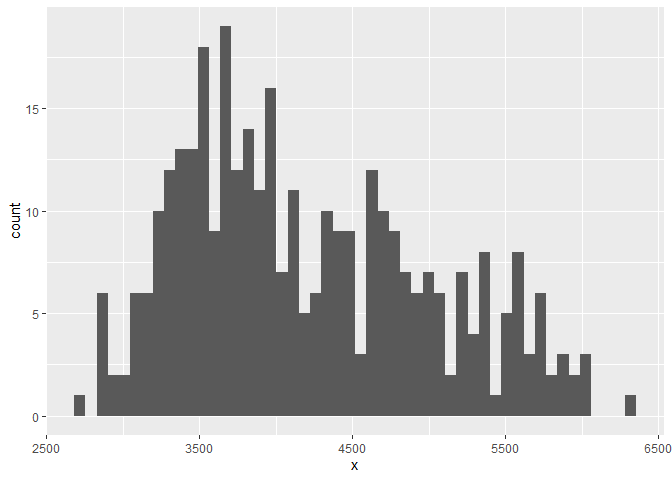
\includegraphics{Final_Proj_files/figure-latex/unnamed-chunk-6-1.pdf}

\begin{quote}
The marriage trends among the different age groups of individuals who
obtained only a high school diploma or less are significant. From 1960
to 2010, individuals age ranged from twenty-five to thirty-four years
old experienced the highest increase of marraige trend followed by
thirty-five to fourty-four years olds, then fourty-five to fifty-four
years old. The marriage trend for all three groups started gaining
traction starting in 1980 with the orange age group exponentially
increased their marriage rate trend when compared to other group's
marriage trend. Overall, the older an individual who only has a high
school diploma is, the lower the chance of them marrying, but marriage
rate for every age group is still increasing throughout the years.
\end{quote}

\hypertarget{women-marriage-data-for-individuals-with-only-a-high-school-diploma-and-less.}{%
\subsubsection{women Marriage Data for individuals with only a high
school diploma and
less.}\label{women-marriage-data-for-individuals-with-only-a-high-school-diploma-and-less.}}

\begin{Shaded}
\begin{Highlighting}[]
\NormalTok{w }\OtherTok{\textless{}{-}}\NormalTok{ women\_data }\SpecialCharTok{\%\textgreater{}\%}
  \FunctionTok{select}\NormalTok{(year, }\FunctionTok{starts\_with}\NormalTok{(}\StringTok{"HS\_"}\NormalTok{)) }

\NormalTok{w\_long }\OtherTok{\textless{}{-}}\NormalTok{ w }\SpecialCharTok{\%\textgreater{}\%} \FunctionTok{pivot\_longer}\NormalTok{(}
  \AttributeTok{cols =} \SpecialCharTok{{-}}\NormalTok{year,}
  \AttributeTok{names\_sep =} \StringTok{"\_"}\NormalTok{,}
  \AttributeTok{names\_to =} \FunctionTok{c}\NormalTok{(}\StringTok{"edu"}\NormalTok{, }\StringTok{"age"}\NormalTok{),}
  \AttributeTok{values\_to =} \StringTok{"rate"}
\NormalTok{)}

\NormalTok{w\_long\_trim }\OtherTok{\textless{}{-}} 
\NormalTok{  w\_long }\SpecialCharTok{\%\textgreater{}\%} 
  \FunctionTok{mutate}\NormalTok{(}\AttributeTok{age\_range =} \FunctionTok{case\_when}\NormalTok{(}
\NormalTok{    age }\SpecialCharTok{==} \StringTok{"2534"} \SpecialCharTok{\textasciitilde{}} \StringTok{"25 to 34"}\NormalTok{,}
\NormalTok{    age }\SpecialCharTok{==} \StringTok{"3544"} \SpecialCharTok{\textasciitilde{}} \StringTok{"35 to 44"}\NormalTok{,}
\NormalTok{    age }\SpecialCharTok{==} \StringTok{"4554"} \SpecialCharTok{\textasciitilde{}} \StringTok{"45 to 54"}
\NormalTok{  ))}

\NormalTok{w\_plot }\OtherTok{\textless{}{-}}\NormalTok{ w\_long\_trim }\SpecialCharTok{\%\textgreater{}\%} 
  \FunctionTok{ggplot}\NormalTok{(}\FunctionTok{aes}\NormalTok{(}
    \AttributeTok{x=}\NormalTok{year,}
    \AttributeTok{y=}\NormalTok{rate,}
    \AttributeTok{color =}\NormalTok{ age\_range)) }\SpecialCharTok{+}
  \FunctionTok{geom\_point}\NormalTok{() }\SpecialCharTok{+}
  \FunctionTok{geom\_smooth}\NormalTok{(}
    \AttributeTok{method =} \StringTok{"lm"}\NormalTok{,}
    \AttributeTok{se =} \ConstantTok{FALSE}\NormalTok{) }\SpecialCharTok{+}
  \FunctionTok{labs}\NormalTok{(}\AttributeTok{title =} \StringTok{"Marriage Trend Amongst Different Age Group Over Time for Women with only High School Diploma."}\NormalTok{,}
    \AttributeTok{x =} \StringTok{"year"}\NormalTok{,}
    \AttributeTok{y =} \StringTok{"Marriage Rate"}\NormalTok{,}
    \AttributeTok{color =} \StringTok{"Age Range:"}
\NormalTok{  ) }\SpecialCharTok{+}
   \FunctionTok{theme\_minimal}\NormalTok{() }\SpecialCharTok{+}
  \FunctionTok{theme}\NormalTok{(}
    \AttributeTok{legend.position =} \StringTok{"right"}\NormalTok{)}

\NormalTok{w\_plot}
\end{Highlighting}
\end{Shaded}

\begin{verbatim}
## `geom_smooth()` using formula 'y ~ x'
\end{verbatim}

\includegraphics{Final_Proj_files/figure-latex/unnamed-chunk-7-1.pdf}

\begin{quote}
Overall, the trend of marriage rate for women also matches up with the
men, although the rate is not as high. The increasing pattern is similar
that of the men with the noticeable increase in the trend starting in
the 1990s.
\end{quote}

\hypertarget{comparing-graphs-of-marriage-trend-for-men-and-women-who-only-have-a-high-school-diploma-or-less.}{%
\subsection{Comparing graphs of marriage trend for men and women who
only have a high school diploma or
less.}\label{comparing-graphs-of-marriage-trend-for-men-and-women-who-only-have-a-high-school-diploma-or-less.}}

\begin{Shaded}
\begin{Highlighting}[]
\NormalTok{combined\_w\_m\_plot }\OtherTok{\textless{}{-}}\NormalTok{ m\_plot }\SpecialCharTok{+}\NormalTok{ w\_plot}
\NormalTok{combined\_w\_m\_plot}
\end{Highlighting}
\end{Shaded}

\begin{verbatim}
## `geom_smooth()` using formula 'y ~ x'
## `geom_smooth()` using formula 'y ~ x'
\end{verbatim}

\includegraphics{Final_Proj_files/figure-latex/unnamed-chunk-8-1.pdf}

\begin{quote}
The comparative visual above is a better look into the comparison of the
trends between two genders.
\end{quote}

\begin{Shaded}
\begin{Highlighting}[]
\FunctionTok{ggsave}\NormalTok{(here}\SpecialCharTok{::}\FunctionTok{here}\NormalTok{(}\StringTok{"Final\_project"}\NormalTok{, }\StringTok{"output"}\NormalTok{, }\StringTok{"figure"}\NormalTok{,}
                  \StringTok{"Marriage Trend Amongst Different Age Group Over Time for Men with High School diploma or less.svg"}\NormalTok{),}
\NormalTok{       m\_plot,}
       \AttributeTok{height =} \DecValTok{6}\NormalTok{,}
       \AttributeTok{width =} \DecValTok{6}\NormalTok{)}
\end{Highlighting}
\end{Shaded}

\begin{verbatim}
## `geom_smooth()` using formula 'y ~ x'
\end{verbatim}

\begin{Shaded}
\begin{Highlighting}[]
\FunctionTok{ggsave}\NormalTok{(here}\SpecialCharTok{::}\FunctionTok{here}\NormalTok{(}\StringTok{"Final\_project"}\NormalTok{, }\StringTok{"output"}\NormalTok{, }\StringTok{"figure"}\NormalTok{,}
                  \StringTok{"Marriage Trend Amongst Different Age Group Over Time for Women with High School diploma or less.svg"}\NormalTok{),}
\NormalTok{       w\_plot,}
       \AttributeTok{height =} \DecValTok{10}\NormalTok{,}
       \AttributeTok{width =} \DecValTok{10}\NormalTok{)}
\end{Highlighting}
\end{Shaded}

\begin{verbatim}
## `geom_smooth()` using formula 'y ~ x'
\end{verbatim}

\begin{Shaded}
\begin{Highlighting}[]
\FunctionTok{ggsave}\NormalTok{(here}\SpecialCharTok{::}\FunctionTok{here}\NormalTok{(}\StringTok{"Final\_project"}\NormalTok{, }\StringTok{"output"}\NormalTok{, }\StringTok{"figure"}\NormalTok{,}
                  \StringTok{"Comparative Marriage Trend Amongst Different Age Group Over Time for both gender with High School diploma or less.svg"}\NormalTok{),}
\NormalTok{       combined\_w\_m\_plot,}
       \AttributeTok{height =} \DecValTok{20}\NormalTok{,}
       \AttributeTok{width =} \DecValTok{20}\NormalTok{)}
\end{Highlighting}
\end{Shaded}

\begin{verbatim}
## `geom_smooth()` using formula 'y ~ x'
## `geom_smooth()` using formula 'y ~ x'
\end{verbatim}

\hypertarget{data-summary-of-both-gender-for-individuals-with-a-high-school-diploma-or-less.}{%
\subsection{Data summary of both gender for individuals with a high
school diploma or
less.}\label{data-summary-of-both-gender-for-individuals-with-a-high-school-diploma-or-less.}}

\begin{quote}
First, I want to create a list of all of the age range of individuals
holding a high school diploma or less.
\end{quote}

\begin{Shaded}
\begin{Highlighting}[]
\NormalTok{HS\_all\_age }\OtherTok{\textless{}{-}}\NormalTok{ both\_gender }\SpecialCharTok{\%\textgreater{}\%} 
  \FunctionTok{select}\NormalTok{(}\FunctionTok{c}\NormalTok{(}
    \StringTok{"year"}\NormalTok{,}
    \StringTok{"HS\_2534"}\NormalTok{,}
    \StringTok{"HS\_3544"}\NormalTok{,}
    \StringTok{"HS\_4554"}\NormalTok{))}
\end{Highlighting}
\end{Shaded}

\begin{quote}
Then I calculated the data.
\end{quote}

\begin{Shaded}
\begin{Highlighting}[]
\NormalTok{sum\_for\_both\_gend }\OtherTok{\textless{}{-}}\NormalTok{ HS\_all\_age }\SpecialCharTok{\%\textgreater{}\%} 
  \FunctionTok{group\_by}\NormalTok{(year) }\SpecialCharTok{\%\textgreater{}\%} 
  \FunctionTok{summarise\_all}\NormalTok{(}
    \FunctionTok{funs}\NormalTok{(}\FunctionTok{n}\NormalTok{(),}
\NormalTok{         mean,}
\NormalTok{         median))}
\end{Highlighting}
\end{Shaded}

\begin{verbatim}
## Warning: `funs()` is deprecated as of dplyr 0.8.0.
## Please use a list of either functions or lambdas: 
## 
##   # Simple named list: 
##   list(mean = mean, median = median)
## 
##   # Auto named with `tibble::lst()`: 
##   tibble::lst(mean, median)
## 
##   # Using lambdas
##   list(~ mean(., trim = .2), ~ median(., na.rm = TRUE))
## This warning is displayed once every 8 hours.
## Call `lifecycle::last_warnings()` to see where this warning was generated.
\end{verbatim}

\begin{Shaded}
\begin{Highlighting}[]
\NormalTok{sum\_for\_both\_gend}
\end{Highlighting}
\end{Shaded}

\begin{verbatim}
## # A tibble: 17 x 10
##     year HS_2534_n HS_3544_n HS_4554_n HS_2534_mean HS_3544_mean HS_4554_mean
##  * <int>     <int>     <int>     <int>        <dbl>        <dbl>        <dbl>
##  1  1960         1         1         1        0.110       0.0686       0.0684
##  2  1970         1         1         1        0.109       0.0651       0.0583
##  3  1980         1         1         1        0.162       0.0643       0.0504
##  4  1990         1         1         1        0.278       0.112        0.0599
##  5  2000         1         1         1        0.332       0.170        0.0944
##  6  2001         1         1         1        0.345       0.169        0.0919
##  7  2002         1         1         1        0.349       0.170        0.0964
##  8  2003         1         1         1        0.358       0.174        0.102 
##  9  2004         1         1         1        0.371       0.182        0.108 
## 10  2005         1         1         1        0.387       0.187        0.115 
## 11  2006         1         1         1        0.431       0.221        0.138 
## 12  2007         1         1         1        0.444       0.226        0.140 
## 13  2008         1         1         1        0.460       0.235        0.154 
## 14  2009         1         1         1        0.485       0.247        0.158 
## 15  2010         1         1         1        0.494       0.253        0.164 
## 16  2011         1         1         1        0.512       0.263        0.170 
## 17  2012         1         1         1        0.524       0.269        0.170 
## # ... with 3 more variables: HS_2534_median <dbl>, HS_3544_median <dbl>,
## #   HS_4554_median <dbl>
\end{verbatim}

\begin{Shaded}
\begin{Highlighting}[]
\FunctionTok{write.csv}\NormalTok{(}
\NormalTok{  sum\_for\_both\_gend,}
\NormalTok{          here}\SpecialCharTok{::}\FunctionTok{here}\NormalTok{(}
            \StringTok{"Final\_project"}\NormalTok{,}
            \StringTok{"output"}\NormalTok{,}
            \StringTok{"Sum\_both\_gend.csv"}\NormalTok{))}
\end{Highlighting}
\end{Shaded}

\begin{Shaded}
\begin{Highlighting}[]
\NormalTok{Sum\_both\_gend\_corr }\OtherTok{\textless{}{-}}\NormalTok{ sum\_for\_both\_gend }\SpecialCharTok{\%\textgreater{}\%} 
\NormalTok{  correlation}\SpecialCharTok{::}\FunctionTok{correlation}\NormalTok{(}
    \AttributeTok{select =} \FunctionTok{c}\NormalTok{(}
      \StringTok{"HS\_2534\_mean"}\NormalTok{,}
      \StringTok{"HS\_3544\_mean"}\NormalTok{,}
      \StringTok{"HS\_4554\_mean"}\NormalTok{)) }\SpecialCharTok{\%\textgreater{}\%} 
  \FunctionTok{summary}\NormalTok{()}

\NormalTok{both\_gend\_tab }\OtherTok{\textless{}{-}} \FunctionTok{full\_join}\NormalTok{(}
\NormalTok{  sum\_for\_both\_gend,}
\NormalTok{  Sum\_both\_gend\_corr)}
\end{Highlighting}
\end{Shaded}

\begin{verbatim}
## Joining, by = c("HS_3544_mean", "HS_4554_mean")
\end{verbatim}

\begin{Shaded}
\begin{Highlighting}[]
\NormalTok{both\_gend\_tab}
\end{Highlighting}
\end{Shaded}

\begin{verbatim}
## # A tibble: 19 x 11
##     year HS_2534_n HS_3544_n HS_4554_n HS_2534_mean HS_3544_mean HS_4554_mean
##    <int>     <int>     <int>     <int>        <dbl>        <dbl>        <dbl>
##  1  1960         1         1         1        0.110       0.0686       0.0684
##  2  1970         1         1         1        0.109       0.0651       0.0583
##  3  1980         1         1         1        0.162       0.0643       0.0504
##  4  1990         1         1         1        0.278       0.112        0.0599
##  5  2000         1         1         1        0.332       0.170        0.0944
##  6  2001         1         1         1        0.345       0.169        0.0919
##  7  2002         1         1         1        0.349       0.170        0.0964
##  8  2003         1         1         1        0.358       0.174        0.102 
##  9  2004         1         1         1        0.371       0.182        0.108 
## 10  2005         1         1         1        0.387       0.187        0.115 
## 11  2006         1         1         1        0.431       0.221        0.138 
## 12  2007         1         1         1        0.444       0.226        0.140 
## 13  2008         1         1         1        0.460       0.235        0.154 
## 14  2009         1         1         1        0.485       0.247        0.158 
## 15  2010         1         1         1        0.494       0.253        0.164 
## 16  2011         1         1         1        0.512       0.263        0.170 
## 17  2012         1         1         1        0.524       0.269        0.170 
## 18    NA        NA        NA        NA       NA           0.989        0.935 
## 19    NA        NA        NA        NA       NA          NA            0.969 
## # ... with 4 more variables: HS_2534_median <dbl>, HS_3544_median <dbl>,
## #   HS_4554_median <dbl>, Parameter <chr>
\end{verbatim}

\begin{Shaded}
\begin{Highlighting}[]
\FunctionTok{write.csv}\NormalTok{(both\_gend\_tab,}
\NormalTok{          here}\SpecialCharTok{::}\FunctionTok{here}\NormalTok{(}\StringTok{"Final\_project"}\NormalTok{, }\StringTok{"output"}\NormalTok{, }\StringTok{"Both\_Genders\_Marriage\_Table\_Data\_for\_HS\_output.csv"}\NormalTok{))}
\end{Highlighting}
\end{Shaded}

\begin{quote}
Hm, this looks really wrong. I am not supposed to get a correlation of
anything higher than .7 realistically speaking. But, the correlation I
provided is my attempt at trying to figure out whether age has any
correlation with marriage rate for both genders for individuals who have
a high school diploma or less. The data (which is extremely flawed and I
need to find a way to update, fix this) indicated there is a strong
correlation between age and marriage rate for individuals with a high
school diploma or less throughout the years.
\end{quote}

\hypertarget{both-gender-dataset-comparison-with-the-individual-gender-dataset.}{%
\subsubsection{Both-Gender Dataset Comparison With the Individual Gender
Dataset.}\label{both-gender-dataset-comparison-with-the-individual-gender-dataset.}}

\begin{quote}
Now, we will look at the dataset for both gender and observe their
marriage trend for individuals with only a high school diploma or less.
To check our two previous datasets and see if the provided combined
dataset of both gender matches with our previous one.
\end{quote}

\begin{Shaded}
\begin{Highlighting}[]
\NormalTok{bg }\OtherTok{\textless{}{-}}\NormalTok{ both\_gender }\SpecialCharTok{\%\textgreater{}\%}
  \FunctionTok{select}\NormalTok{(}
\NormalTok{    year,}
    \FunctionTok{starts\_with}\NormalTok{(}\StringTok{"HS\_"}\NormalTok{)) }


\NormalTok{bg\_long }\OtherTok{\textless{}{-}}\NormalTok{ bg }\SpecialCharTok{\%\textgreater{}\%} 
  \FunctionTok{pivot\_longer}\NormalTok{(}
  \AttributeTok{cols =} \SpecialCharTok{{-}}\NormalTok{year,}
  \AttributeTok{names\_sep =} \StringTok{"\_"}\NormalTok{,}
  \AttributeTok{names\_to =} \FunctionTok{c}\NormalTok{(}\StringTok{"edu"}\NormalTok{, }\StringTok{"age"}\NormalTok{),}
  \AttributeTok{values\_to =} \StringTok{"rate"}
\NormalTok{) }


\NormalTok{bg\_long\_trim }\OtherTok{\textless{}{-}} 
\NormalTok{  bg\_long }\SpecialCharTok{\%\textgreater{}\%} 
  \FunctionTok{mutate}\NormalTok{(}\AttributeTok{age\_range =} \FunctionTok{case\_when}\NormalTok{(}
\NormalTok{    age }\SpecialCharTok{==} \StringTok{"2534"} \SpecialCharTok{\textasciitilde{}} \StringTok{"25 to 34"}\NormalTok{,}
\NormalTok{    age }\SpecialCharTok{==} \StringTok{"3544"} \SpecialCharTok{\textasciitilde{}} \StringTok{"35 to 44"}\NormalTok{,}
\NormalTok{    age }\SpecialCharTok{==} \StringTok{"4554"} \SpecialCharTok{\textasciitilde{}} \StringTok{"45 to 54"}
\NormalTok{  ))}

\NormalTok{bg\_plot }\OtherTok{\textless{}{-}}\NormalTok{ bg\_long\_trim }\SpecialCharTok{\%\textgreater{}\%} 
  \FunctionTok{ggplot}\NormalTok{(}\FunctionTok{aes}\NormalTok{(}\AttributeTok{x=}\NormalTok{year,}\AttributeTok{y=}\NormalTok{rate, }\AttributeTok{color =}\NormalTok{ age\_range)) }\SpecialCharTok{+}
  \FunctionTok{geom\_point}\NormalTok{() }\SpecialCharTok{+}
  \FunctionTok{geom\_smooth}\NormalTok{(}\AttributeTok{method =} \StringTok{"lm"}\NormalTok{, }\AttributeTok{se =} \ConstantTok{FALSE}\NormalTok{) }\SpecialCharTok{+}
  \FunctionTok{scale\_color\_brewer}\NormalTok{(}\AttributeTok{palette =} \StringTok{"YlOrRd"}\NormalTok{) }\SpecialCharTok{+}
  \FunctionTok{labs}\NormalTok{(}
    \AttributeTok{title =} \StringTok{"Marriage Trend Amongst Different Age Group Over Time for Men and Women with only High School Diploma."}\NormalTok{,}
    \AttributeTok{x =} \StringTok{"year"}\NormalTok{,}
    \AttributeTok{y =} \StringTok{"Marriage Rate"}\NormalTok{,}
    \AttributeTok{color =} \StringTok{"Age Range:"}
\NormalTok{  ) }\SpecialCharTok{+}
  \FunctionTok{theme\_minimal}\NormalTok{() }\SpecialCharTok{+}
  \FunctionTok{theme}\NormalTok{(}\AttributeTok{legend.position =} \StringTok{"right"}\NormalTok{)}


\NormalTok{bg\_plot}
\end{Highlighting}
\end{Shaded}

\begin{verbatim}
## `geom_smooth()` using formula 'y ~ x'
\end{verbatim}

\includegraphics{Final_Proj_files/figure-latex/unnamed-chunk-13-1.pdf}

\begin{Shaded}
\begin{Highlighting}[]
\FunctionTok{ggsave}\NormalTok{(here}\SpecialCharTok{::}\FunctionTok{here}\NormalTok{(}\StringTok{"Final\_project"}\NormalTok{,}
                  \StringTok{"output"}\NormalTok{,}
                  \StringTok{"figure"}\NormalTok{,}
                  \StringTok{"Marriage Trend Amongst Different Age Group Over Time for both gender with High School diploma or less.svg"}\NormalTok{),}
\NormalTok{       bg\_plot,}
       \AttributeTok{height =} \DecValTok{10}\NormalTok{,}
       \AttributeTok{width =} \DecValTok{10}\NormalTok{)}
\end{Highlighting}
\end{Shaded}

\begin{verbatim}
## `geom_smooth()` using formula 'y ~ x'
\end{verbatim}

\begin{quote}
This dataset seems very similar to the two individually produced
gendered datasets mentioned above.
\end{quote}

\begin{Shaded}
\begin{Highlighting}[]
\NormalTok{main\_compared\_data }\OtherTok{\textless{}{-}}\NormalTok{ m\_plot }\SpecialCharTok{+}\NormalTok{ w\_plot }\SpecialCharTok{+}\NormalTok{ bg\_plot}
\NormalTok{main\_compared\_data}
\end{Highlighting}
\end{Shaded}

\begin{verbatim}
## `geom_smooth()` using formula 'y ~ x'
## `geom_smooth()` using formula 'y ~ x'
## `geom_smooth()` using formula 'y ~ x'
\end{verbatim}

\includegraphics{Final_Proj_files/figure-latex/unnamed-chunk-14-1.pdf}

\begin{Shaded}
\begin{Highlighting}[]
\FunctionTok{ggsave}\NormalTok{(}
\NormalTok{  here}\SpecialCharTok{::}\FunctionTok{here}\NormalTok{(}
    \StringTok{"Final\_project"}\NormalTok{,}
    \StringTok{"output"}\NormalTok{,}
    \StringTok{"figure"}\NormalTok{,}
    \StringTok{"Comparison of Marriage Trend of Men and Women versus Combined who only have High School Diploma.svg"}\NormalTok{),}
\NormalTok{  main\_compared\_data,}
  \AttributeTok{height =} \DecValTok{25}\NormalTok{,}
  \AttributeTok{width =} \DecValTok{25}\NormalTok{)}
\end{Highlighting}
\end{Shaded}

\begin{verbatim}
## `geom_smooth()` using formula 'y ~ x'
## `geom_smooth()` using formula 'y ~ x'
## `geom_smooth()` using formula 'y ~ x'
\end{verbatim}

\begin{quote}
At this rate, it can be safely assumed that the dataset with both gender
approximately matches with the two individual gender dataset. WE will
use the dataset with both genders in the future due to its conveinency
for future comparison with divorce rate, etc.
\end{quote}

\begin{quote}
We are going to transform the ``Both gender'' dataset into a Tibble here
and save everytihng.
\end{quote}

\begin{Shaded}
\begin{Highlighting}[]
\NormalTok{tibble\_both\_gender }\OtherTok{\textless{}{-}} \FunctionTok{as.tibble}\NormalTok{(}
\NormalTok{  both\_gender)}
\end{Highlighting}
\end{Shaded}

\begin{verbatim}
## Warning: `as.tibble()` is deprecated as of tibble 2.0.0.
## Please use `as_tibble()` instead.
## The signature and semantics have changed, see `?as_tibble`.
## This warning is displayed once every 8 hours.
## Call `lifecycle::last_warnings()` to see where this warning was generated.
\end{verbatim}

\begin{Shaded}
\begin{Highlighting}[]
\FunctionTok{print}\NormalTok{(tibble\_both\_gender)}
\end{Highlighting}
\end{Shaded}

\begin{verbatim}
## # A tibble: 17 x 75
##        X  year date  all_2534 HS_2534 SC_2534 BAp_2534 BAo_2534 GD_2534
##    <int> <int> <chr>    <dbl>   <dbl>   <dbl>    <dbl>    <dbl>   <dbl>
##  1     1  1960 1960~    0.123   0.110   0.152    0.239    0.239  NA    
##  2     2  1970 1970~    0.127   0.109   0.150    0.219    0.219  NA    
##  3     3  1980 1980~    0.199   0.162   0.224    0.288    0.288  NA    
##  4     4  1990 1990~    0.297   0.278   0.278    0.361    0.366   0.347
##  5     5  2000 2000~    0.345   0.332   0.325    0.387    0.394   0.369
##  6     6  2001 2001~    0.353   0.345   0.334    0.384    0.393   0.359
##  7     7  2002 2002~    0.354   0.349   0.336    0.377    0.387   0.351
##  8     8  2003 2003~    0.362   0.358   0.342    0.387    0.400   0.354
##  9     9  2004 2004~    0.367   0.371   0.345    0.385    0.398   0.352
## 10    10  2005 2005~    0.379   0.387   0.360    0.389    0.403   0.351
## 11    11  2006 2006~    0.415   0.431   0.391    0.415    0.430   0.376
## 12    12  2007 2007~    0.427   0.444   0.408    0.421    0.439   0.375
## 13    13  2008 2008~    0.439   0.460   0.424    0.430    0.447   0.385
## 14    14  2009 2009~    0.463   0.485   0.447    0.452    0.474   0.396
## 15    15  2010 2010~    0.470   0.494   0.454    0.456    0.477   0.406
## 16    16  2011 2011~    0.483   0.512   0.469    0.466    0.490   0.407
## 17    17  2012 2012~    0.494   0.524   0.480    0.477    0.502   0.416
## # ... with 66 more variables: White_2534 <dbl>, Black_2534 <dbl>,
## #   Hisp_2534 <dbl>, NE_2534 <dbl>, MA_2534 <dbl>, Midwest_2534 <dbl>,
## #   South_2534 <dbl>, Mountain_2534 <dbl>, Pacific_2534 <dbl>, poor_2534 <dbl>,
## #   mid_2534 <dbl>, rich_2534 <dbl>, all_3544 <dbl>, HS_3544 <dbl>,
## #   SC_3544 <dbl>, BAp_3544 <dbl>, BAo_3544 <dbl>, GD_3544 <dbl>,
## #   White_3544 <dbl>, Black_3544 <dbl>, Hisp_3544 <dbl>, NE_3544 <dbl>,
## #   MA_3544 <dbl>, Midwest_3544 <dbl>, South_3544 <dbl>, Mountain_3544 <dbl>,
## #   Pacific_3544 <dbl>, poor_3544 <dbl>, mid_3544 <dbl>, rich_3544 <dbl>,
## #   all_4554 <dbl>, HS_4554 <dbl>, SC_4554 <dbl>, BAp_4554 <dbl>,
## #   BAo_4554 <dbl>, GD_4554 <dbl>, White_4554 <dbl>, Black_4554 <dbl>,
## #   Hisp_4554 <dbl>, NE_4554 <dbl>, MA_4554 <dbl>, Midwest_4554 <dbl>,
## #   South_4554 <dbl>, Mountain_4554 <dbl>, Pacific_4554 <dbl>, poor_4554 <dbl>,
## #   mid_4554 <dbl>, rich_4554 <dbl>, nokids_all_2534 <dbl>,
## #   kids_all_2534 <dbl>, nokids_HS_2534 <dbl>, nokids_SC_2534 <dbl>,
## #   nokids_BAp_2534 <dbl>, nokids_BAo_2534 <dbl>, nokids_GD_2534 <dbl>,
## #   kids_HS_2534 <dbl>, kids_SC_2534 <dbl>, kids_BAp_2534 <dbl>,
## #   kids_BAo_2534 <dbl>, kids_GD_2534 <dbl>, nokids_poor_2534 <dbl>,
## #   nokids_mid_2534 <dbl>, nokids_rich_2534 <dbl>, kids_poor_2534 <dbl>,
## #   kids_mid_2534 <dbl>, kids_rich_2534 <dbl>
\end{verbatim}

\begin{Shaded}
\begin{Highlighting}[]
\FunctionTok{write.csv}\NormalTok{(tibble\_both\_gender, }
\NormalTok{          here}\SpecialCharTok{::}\FunctionTok{here}\NormalTok{(}
            \StringTok{"Final\_project"}\NormalTok{,}
            \StringTok{"data"}\NormalTok{,}
            \StringTok{"tibble\_both\_gender.csv"}\NormalTok{))}
\end{Highlighting}
\end{Shaded}

\begin{Shaded}
\begin{Highlighting}[]
\FunctionTok{write.csv}\NormalTok{(m\_long\_trim,}
\NormalTok{          here}\SpecialCharTok{::}\FunctionTok{here}\NormalTok{(}\StringTok{"Final\_project"}\NormalTok{, }\StringTok{"output"}\NormalTok{, }\StringTok{"Men\_Marriage\_Rate\_Trimmed\_for\_HS\_output.csv"}\NormalTok{))}
\FunctionTok{write.csv}\NormalTok{(w\_long\_trim,}
\NormalTok{          here}\SpecialCharTok{::}\FunctionTok{here}\NormalTok{(}\StringTok{"Final\_project"}\NormalTok{, }\StringTok{"output"}\NormalTok{, }\StringTok{"Women\_Marriage\_Rate\_Trimmed\_for\_HS\_output.csv"}\NormalTok{))}
\FunctionTok{write.csv}\NormalTok{(bg\_long\_trim,}
\NormalTok{          here}\SpecialCharTok{::}\FunctionTok{here}\NormalTok{(}\StringTok{"Final\_project"}\NormalTok{, }\StringTok{"output"}\NormalTok{, }\StringTok{"Both\_Genders\_Marriage\_Rate\_Trimmed\_for\_HS\_output.csv"}\NormalTok{))}
\end{Highlighting}
\end{Shaded}

\hypertarget{marriage-rate-and-trend-of-individuals-with-a-bachelor-degree-or-higher.}{%
\subsubsection{Marriage Rate and Trend of Individuals with a Bachelor
Degree or
higher.}\label{marriage-rate-and-trend-of-individuals-with-a-bachelor-degree-or-higher.}}

\begin{quote}
Let's calculate the maximum output for individuals with a Bachelor or
higher.
\end{quote}

\begin{Shaded}
\begin{Highlighting}[]
\NormalTok{tibble\_both\_gender\_output1 }\OtherTok{\textless{}{-}}\NormalTok{ tibble\_both\_gender }\SpecialCharTok{\%\textgreater{}\%}
  \FunctionTok{select}\NormalTok{(}
\NormalTok{    year,}
\NormalTok{    date,}
\NormalTok{    BAp\_2534) }\SpecialCharTok{\%\textgreater{}\%} 
  \FunctionTok{group\_by}\NormalTok{(year) }\SpecialCharTok{\%\textgreater{}\%}
  \FunctionTok{filter}\NormalTok{(}
\NormalTok{    BAp\_2534 }\SpecialCharTok{==} \FunctionTok{max}\NormalTok{(BAp\_2534))}

\NormalTok{tibble\_both\_gender\_output1}
\end{Highlighting}
\end{Shaded}

\begin{verbatim}
## # A tibble: 17 x 3
## # Groups:   year [17]
##     year date       BAp_2534
##    <int> <chr>         <dbl>
##  1  1960 1960-01-01    0.239
##  2  1970 1970-01-01    0.219
##  3  1980 1980-01-01    0.288
##  4  1990 1990-01-01    0.361
##  5  2000 2000-01-01    0.387
##  6  2001 2001-01-01    0.384
##  7  2002 2002-01-01    0.377
##  8  2003 2003-01-01    0.387
##  9  2004 2004-01-01    0.385
## 10  2005 2005-01-01    0.389
## 11  2006 2006-01-01    0.415
## 12  2007 2007-01-01    0.421
## 13  2008 2008-01-01    0.430
## 14  2009 2009-01-01    0.452
## 15  2010 2010-01-01    0.456
## 16  2011 2011-01-01    0.466
## 17  2012 2012-01-01    0.477
\end{verbatim}

\begin{Shaded}
\begin{Highlighting}[]
\FunctionTok{write.csv}\NormalTok{(tibble\_both\_gender\_output1,}
\NormalTok{          here}\SpecialCharTok{::}\FunctionTok{here}\NormalTok{(}\StringTok{"Final\_project"}\NormalTok{, }\StringTok{"output"}\NormalTok{, }\StringTok{"Max\_change\_in\_years\_for\_higher\_education.csv"}\NormalTok{))}
\end{Highlighting}
\end{Shaded}

\begin{quote}
As we can see here, the maximum marriage population for people with
higher level of education seems to increase over time. This of course is
just one variable.
\end{quote}

\begin{quote}
Let's create a graph to observe the marriage trend of individuals
possessing a Bachelor or higher.
\end{quote}

\begin{Shaded}
\begin{Highlighting}[]
\NormalTok{bg\_Bach\_high }\OtherTok{\textless{}{-}}\NormalTok{ both\_gender }\SpecialCharTok{\%\textgreater{}\%}
  \FunctionTok{select}\NormalTok{(year, }\FunctionTok{starts\_with}\NormalTok{(}\FunctionTok{c}\NormalTok{(}\StringTok{"BAo\_"}\NormalTok{, }\StringTok{"BAp\_"}\NormalTok{))) }

\NormalTok{bg\_Bach\_high\_long }\OtherTok{\textless{}{-}}\NormalTok{ bg\_Bach\_high }\SpecialCharTok{\%\textgreater{}\%} 
  \FunctionTok{pivot\_longer}\NormalTok{(}
  \AttributeTok{cols =} \SpecialCharTok{{-}}\NormalTok{year,}
  \AttributeTok{names\_sep =} \StringTok{"\_"}\NormalTok{,}
  \AttributeTok{names\_to =} \FunctionTok{c}\NormalTok{(}\StringTok{"edu"}\NormalTok{, }\StringTok{"age"}\NormalTok{),}
  \AttributeTok{values\_to =} \StringTok{"rate"}
\NormalTok{)}

\NormalTok{bg\_Bach\_high\_long\_trim }\OtherTok{\textless{}{-}} 
\NormalTok{  bg\_Bach\_high\_long }\SpecialCharTok{\%\textgreater{}\%} 
  \FunctionTok{mutate}\NormalTok{(}\AttributeTok{age\_range =} \FunctionTok{case\_when}\NormalTok{(}
\NormalTok{    age }\SpecialCharTok{==} \StringTok{"2534"} \SpecialCharTok{\textasciitilde{}} \StringTok{"25 to 34"}\NormalTok{,}
\NormalTok{    age }\SpecialCharTok{==} \StringTok{"3544"} \SpecialCharTok{\textasciitilde{}} \StringTok{"35 to 44"}\NormalTok{,}
\NormalTok{    age }\SpecialCharTok{==} \StringTok{"4554"} \SpecialCharTok{\textasciitilde{}} \StringTok{"45 to 54"}
\NormalTok{  ))}

\NormalTok{bg\_Bach\_high\_plot }\OtherTok{\textless{}{-}}\NormalTok{ bg\_Bach\_high\_long\_trim }\SpecialCharTok{\%\textgreater{}\%} 
  \FunctionTok{ggplot}\NormalTok{(}\FunctionTok{aes}\NormalTok{(}
    \AttributeTok{x=}\NormalTok{year,}
    \AttributeTok{y=}\NormalTok{rate,}
    \AttributeTok{color =}\NormalTok{ age\_range)) }\SpecialCharTok{+}
  \FunctionTok{geom\_point}\NormalTok{() }\SpecialCharTok{+}
  \FunctionTok{geom\_smooth}\NormalTok{(}
    \AttributeTok{method =} \StringTok{"lm"}\NormalTok{,}
    \AttributeTok{se =} \ConstantTok{FALSE}\NormalTok{) }\SpecialCharTok{+}
  \FunctionTok{scale\_color\_viridis}\NormalTok{(}
    \AttributeTok{discrete =} \ConstantTok{TRUE}\NormalTok{, }\AttributeTok{option =} \StringTok{"D"}\NormalTok{) }\SpecialCharTok{+}
  \FunctionTok{scale\_fill\_viridis}\NormalTok{(}
    \AttributeTok{discrete =} \ConstantTok{TRUE}\NormalTok{) }\SpecialCharTok{+}
  \FunctionTok{labs}\NormalTok{(}\AttributeTok{title =} \StringTok{"Marriage Trend Amongst Different Age Group Over Time for Men and Women with Bachelor or Higher."}\NormalTok{, }
       \AttributeTok{x =} \StringTok{"year"}\NormalTok{, }
       \AttributeTok{y =} \StringTok{"Marriage Rate"}\NormalTok{,}
       \AttributeTok{color =} \StringTok{"Age Range:"}\NormalTok{) }\SpecialCharTok{+}
  \FunctionTok{theme\_minimal}\NormalTok{() }\SpecialCharTok{+}
  \FunctionTok{theme}\NormalTok{(}\AttributeTok{legend.position =} \StringTok{"top"}\NormalTok{)}

\NormalTok{bg\_Bach\_high\_plot}
\end{Highlighting}
\end{Shaded}

\begin{verbatim}
## `geom_smooth()` using formula 'y ~ x'
\end{verbatim}

\includegraphics{Final_Proj_files/figure-latex/unnamed-chunk-18-1.pdf}

\begin{quote}
Compared to the marriage rate of individuals who have lower education
than the ones who have a bachelor or higher, It can be seen that the
marriage rate of individuals who are of higher-level-of-education are
not marrying as much. The trend for these individuals plateau around the
age of 45 to 54 throughout the years with a slight increase starting in
the early 2000s, but plateu and decreased again. The rate of marriage
for individuals with a Bachelor Degree or higher seems to be
significantly less than the ones who only have high school diploma or
less when their age is 35 years old or older. Although higher marriage
rate was observed at the beginning of 1960 for Bachelor Degree or higher
individuals, no significant differences in the marriage trend of
individuals at the age of 25 to 34 can be seen throughhout the years
when education is taken into account. This data can be seen down below.
\end{quote}

\begin{Shaded}
\begin{Highlighting}[]
\FunctionTok{write.csv}\NormalTok{(bg\_Bach\_high\_long\_trim,}
\NormalTok{          here}\SpecialCharTok{::}\FunctionTok{here}\NormalTok{(}
            \StringTok{"Final\_project"}\NormalTok{, }
            \StringTok{"output"}\NormalTok{, }
            \StringTok{"Both\_Genders\_Marriage\_Rate\_Trimmed\_for\_BA\_and\_higher\_output.csv"}\NormalTok{))}
\end{Highlighting}
\end{Shaded}

\begin{quote}
Now, let's observe the trend differences in marriage rate between
individuals with only a high school diploma versus individuals with a
Bachelor or higher.
\end{quote}

\begin{Shaded}
\begin{Highlighting}[]
\NormalTok{comparative\_data\_for\_marriage\_hsBa }\OtherTok{\textless{}{-}}\NormalTok{ bg\_plot }\SpecialCharTok{+}\NormalTok{ bg\_Bach\_high\_plot}

\NormalTok{comparative\_data\_for\_marriage\_hsBa}
\end{Highlighting}
\end{Shaded}

\begin{verbatim}
## `geom_smooth()` using formula 'y ~ x'
## `geom_smooth()` using formula 'y ~ x'
\end{verbatim}

\includegraphics{Final_Proj_files/figure-latex/unnamed-chunk-20-1.pdf}

\begin{Shaded}
\begin{Highlighting}[]
\FunctionTok{ggsave}\NormalTok{(}
\NormalTok{  here}\SpecialCharTok{::}\FunctionTok{here}\NormalTok{(}
    \StringTok{"Final\_project"}\NormalTok{,}
    \StringTok{"output"}\NormalTok{,}
    \StringTok{"figure"}\NormalTok{,}
    \StringTok{"Comparative Data of Marriage Rate for different age groups throughout education level.svg"}\NormalTok{),}
\NormalTok{       comparative\_data\_for\_marriage\_hsBa,}
       \AttributeTok{height =} \DecValTok{25}\NormalTok{,}
       \AttributeTok{width =} \DecValTok{25}\NormalTok{)}
\end{Highlighting}
\end{Shaded}

\begin{verbatim}
## `geom_smooth()` using formula 'y ~ x'
## `geom_smooth()` using formula 'y ~ x'
\end{verbatim}

\begin{quote}
The differences in the trend's growth in different individuals
possessing different education level can be observe here.
\end{quote}

\hypertarget{divorce-rate-calculation.}{%
\subsubsection{Divorce Rate
Calculation.}\label{divorce-rate-calculation.}}

\begin{quote}
Now, let's look at divorce rate among the population throughout the year
by education.
\end{quote}

\begin{Shaded}
\begin{Highlighting}[]
\NormalTok{Divorce\_sum }\OtherTok{\textless{}{-}}\NormalTok{ Major\_data }\SpecialCharTok{\%\textgreater{}\%} 
  \FunctionTok{summarize}\NormalTok{(}\FunctionTok{across}\NormalTok{(}\FunctionTok{c}\NormalTok{(HS\_3544}\SpecialCharTok{:}\NormalTok{BAp\_3544),}
                      \FunctionTok{list}\NormalTok{(}\AttributeTok{mean =} \SpecialCharTok{\textasciitilde{}} \FunctionTok{mean}\NormalTok{(.x, }\AttributeTok{na.rm=} \ConstantTok{TRUE}\NormalTok{),}
                \AttributeTok{sd =} \SpecialCharTok{\textasciitilde{}} \FunctionTok{sd}\NormalTok{(.x, }\AttributeTok{na.rm =} \ConstantTok{TRUE}\NormalTok{),}
                \AttributeTok{min =} \SpecialCharTok{\textasciitilde{}} \FunctionTok{min}\NormalTok{(.x, }\AttributeTok{na.rm =} \ConstantTok{TRUE}\NormalTok{),}
                \AttributeTok{max =} \SpecialCharTok{\textasciitilde{}} \FunctionTok{max}\NormalTok{(.x, }\AttributeTok{na.rm =} \ConstantTok{TRUE}\NormalTok{))))}
\NormalTok{Divorce\_sum}
\end{Highlighting}
\end{Shaded}

\begin{verbatim}
##   HS_3544_mean HS_3544_sd HS_3544_min HS_3544_max SC_3544_mean SC_3544_sd
## 1    0.1601496  0.0488751  0.03488887   0.1923989    0.1633165  0.0500708
##   SC_3544_min SC_3544_max BAp_3544_mean BAp_3544_sd BAp_3544_min BAp_3544_max
## 1  0.03366938   0.2031765    0.09587785  0.02359412   0.02751277    0.1149553
\end{verbatim}

\begin{Shaded}
\begin{Highlighting}[]
\FunctionTok{write.csv}\NormalTok{(}
\NormalTok{  Divorce\_sum,}
\NormalTok{          here}\SpecialCharTok{::}\FunctionTok{here}\NormalTok{(}
            \StringTok{"Final\_project"}\NormalTok{,}
            \StringTok{"output"}\NormalTok{,}
            \StringTok{"Divorce\_sum.csv"}\NormalTok{))}
\end{Highlighting}
\end{Shaded}

\begin{quote}
The divorce summary data was interesting. Let's see if we can observe
the data in a graph form.
\end{quote}

\begin{Shaded}
\begin{Highlighting}[]
\NormalTok{div }\OtherTok{\textless{}{-}}\NormalTok{ Major\_data }\SpecialCharTok{\%\textgreater{}\%}
  \FunctionTok{select}\NormalTok{(year, }\FunctionTok{starts\_with}\NormalTok{(}\StringTok{"HS\_"}\NormalTok{)) }

\NormalTok{div\_long }\OtherTok{\textless{}{-}}\NormalTok{ div }\SpecialCharTok{\%\textgreater{}\%} 
  \FunctionTok{pivot\_longer}\NormalTok{(}
  \AttributeTok{cols =} \SpecialCharTok{{-}}\NormalTok{year,}
  \AttributeTok{names\_sep =} \StringTok{"\_"}\NormalTok{,}
  \AttributeTok{names\_to =} \FunctionTok{c}\NormalTok{(}\StringTok{"edu"}\NormalTok{, }\StringTok{"age"}\NormalTok{),}
  \AttributeTok{values\_to =} \StringTok{"rate"}
\NormalTok{)}

\NormalTok{div\_long\_trim }\OtherTok{\textless{}{-}} 
\NormalTok{  div\_long }\SpecialCharTok{\%\textgreater{}\%} 
  \FunctionTok{mutate}\NormalTok{(}\AttributeTok{age\_range =} \FunctionTok{case\_when}\NormalTok{(}
\NormalTok{    age }\SpecialCharTok{==} \StringTok{"2534"} \SpecialCharTok{\textasciitilde{}} \StringTok{"25 to 34"}\NormalTok{,}
\NormalTok{    age }\SpecialCharTok{==} \StringTok{"3544"} \SpecialCharTok{\textasciitilde{}} \StringTok{"35 to 44"}\NormalTok{,}
\NormalTok{    age }\SpecialCharTok{==} \StringTok{"4554"} \SpecialCharTok{\textasciitilde{}} \StringTok{"45 to 54"}
\NormalTok{  ))}

\NormalTok{div\_plot }\OtherTok{\textless{}{-}}\NormalTok{ div\_long\_trim }\SpecialCharTok{\%\textgreater{}\%} 
  \FunctionTok{ggplot}\NormalTok{(}\FunctionTok{aes}\NormalTok{(}\AttributeTok{x=}\NormalTok{year,}\AttributeTok{y=}\NormalTok{rate, }\AttributeTok{color =}\NormalTok{ age\_range)) }\SpecialCharTok{+}
  \FunctionTok{geom\_point}\NormalTok{() }\SpecialCharTok{+}
  \FunctionTok{geom\_smooth}\NormalTok{(}\AttributeTok{method =} \StringTok{"lm"}\NormalTok{, }\AttributeTok{se =} \ConstantTok{FALSE}\NormalTok{) }\SpecialCharTok{+}
  \FunctionTok{labs}\NormalTok{(}\AttributeTok{title =} \StringTok{"Divorce Trend Among Individuals with only a High School Diploma."}\NormalTok{,}
       \AttributeTok{x =} \StringTok{"Year"}\NormalTok{,}
       \AttributeTok{y =} \StringTok{"Divorce Rate"}\NormalTok{,}
       \AttributeTok{color =} \StringTok{"Age Range:"}\NormalTok{) }\SpecialCharTok{+}
   \FunctionTok{theme\_minimal}\NormalTok{()}\SpecialCharTok{+}
  \FunctionTok{theme}\NormalTok{(}\AttributeTok{legend.position =} \StringTok{"bottom"}\NormalTok{)}

\NormalTok{div\_plot}
\end{Highlighting}
\end{Shaded}

\begin{verbatim}
## `geom_smooth()` using formula 'y ~ x'
\end{verbatim}

\includegraphics{Final_Proj_files/figure-latex/unnamed-chunk-22-1.pdf}

\begin{Shaded}
\begin{Highlighting}[]
\FunctionTok{ggsave}\NormalTok{(}
\NormalTok{  here}\SpecialCharTok{::}\FunctionTok{here}\NormalTok{(}
    \StringTok{"Final\_project"}\NormalTok{, }
    \StringTok{"output"}\NormalTok{, }
    \StringTok{"figure"}\NormalTok{,}
    \StringTok{"Divorce Rate Trend Graph for Individuals possessing a high school diploma or less.svg"}\NormalTok{),}
\NormalTok{       div\_plot,}
       \AttributeTok{height =} \DecValTok{10}\NormalTok{,}
       \AttributeTok{width =} \DecValTok{10}\NormalTok{)}
\end{Highlighting}
\end{Shaded}

\begin{verbatim}
## `geom_smooth()` using formula 'y ~ x'
\end{verbatim}

\begin{quote}
As observed, the divorce trend for individuals with only a high school
diploma is significantly different from the marriage trend with the
difference being the rate is much higher in divorce than in marriage.
Furthermore, the trend is growing even more starting from the early
2000s.
\end{quote}

\begin{Shaded}
\begin{Highlighting}[]
\FunctionTok{write.csv}\NormalTok{(}
\NormalTok{  div\_long\_trim,}
\NormalTok{          here}\SpecialCharTok{::}\FunctionTok{here}\NormalTok{(}
            \StringTok{"Final\_project"}\NormalTok{,}
            \StringTok{"output"}\NormalTok{,}
            \StringTok{"Divorce\_Rate\_Trimmed\_for\_HS\_output.csv"}\NormalTok{))}
\end{Highlighting}
\end{Shaded}

\begin{quote}
Let's calculate divorce rate for individuals with a Bachelor or higher.
\end{quote}

\begin{Shaded}
\begin{Highlighting}[]
\NormalTok{div\_high }\OtherTok{\textless{}{-}}\NormalTok{ Major\_data }\SpecialCharTok{\%\textgreater{}\%}
   \FunctionTok{select}\NormalTok{(year, }\FunctionTok{starts\_with}\NormalTok{(}\FunctionTok{c}\NormalTok{(}\StringTok{"BAo\_"}\NormalTok{, }\StringTok{"BAp\_"}\NormalTok{)))}

\NormalTok{div\_high\_long }\OtherTok{\textless{}{-}}\NormalTok{ div\_high }\SpecialCharTok{\%\textgreater{}\%} 
  \FunctionTok{pivot\_longer}\NormalTok{(}
  \AttributeTok{cols =} \SpecialCharTok{{-}}\NormalTok{year,}
  \AttributeTok{names\_sep =} \StringTok{"\_"}\NormalTok{,}
  \AttributeTok{names\_to =} \FunctionTok{c}\NormalTok{(}\StringTok{"edu"}\NormalTok{, }\StringTok{"age"}\NormalTok{),}
  \AttributeTok{values\_to =} \StringTok{"rate"}
\NormalTok{)}


\NormalTok{div\_high\_long\_trim }\OtherTok{\textless{}{-}} 
\NormalTok{  div\_high\_long }\SpecialCharTok{\%\textgreater{}\%} 
  \FunctionTok{mutate}\NormalTok{(}\AttributeTok{age\_range =} \FunctionTok{case\_when}\NormalTok{(}
\NormalTok{    age }\SpecialCharTok{==} \StringTok{"3544"} \SpecialCharTok{\textasciitilde{}} \StringTok{"35 to 44"}\NormalTok{,}
\NormalTok{    age }\SpecialCharTok{==} \StringTok{"4554"} \SpecialCharTok{\textasciitilde{}} \StringTok{"45 to 54"}
\NormalTok{  ))}

\NormalTok{div\_high\_plot }\OtherTok{\textless{}{-}}\NormalTok{ div\_high\_long\_trim }\SpecialCharTok{\%\textgreater{}\%} 
  \FunctionTok{ggplot}\NormalTok{(}\FunctionTok{aes}\NormalTok{(}
    \AttributeTok{x=}\NormalTok{year,}
    \AttributeTok{y=}\NormalTok{rate,}
    \AttributeTok{color =}\NormalTok{ age\_range)) }\SpecialCharTok{+}
  \FunctionTok{geom\_point}\NormalTok{() }\SpecialCharTok{+}
  \FunctionTok{geom\_smooth}\NormalTok{(}
    \AttributeTok{method =} \StringTok{"lm"}\NormalTok{,}
    \AttributeTok{se =} \ConstantTok{FALSE}\NormalTok{) }\SpecialCharTok{+}
  \FunctionTok{labs}\NormalTok{(}\AttributeTok{title =} \StringTok{"Divorce Trend Among Individuals with Bachelor or Higher."}\NormalTok{,}
       \AttributeTok{x =} \StringTok{"Year"}\NormalTok{,}
       \AttributeTok{y =} \StringTok{"Divorce Rate"}\NormalTok{,}
       \AttributeTok{color =} \StringTok{"Age Range:"}\NormalTok{) }\SpecialCharTok{+}
   \FunctionTok{theme\_minimal}\NormalTok{()}\SpecialCharTok{+}
  \FunctionTok{theme}\NormalTok{(}
    \AttributeTok{legend.position =} \StringTok{"bottom"}\NormalTok{)}

\NormalTok{div\_high\_plot}
\end{Highlighting}
\end{Shaded}

\begin{verbatim}
## `geom_smooth()` using formula 'y ~ x'
\end{verbatim}

\includegraphics{Final_Proj_files/figure-latex/unnamed-chunk-24-1.pdf}

\begin{Shaded}
\begin{Highlighting}[]
\FunctionTok{ggsave}\NormalTok{(}
\NormalTok{  here}\SpecialCharTok{::}\FunctionTok{here}\NormalTok{(}
    \StringTok{"Final\_project"}\NormalTok{, }
    \StringTok{"output"}\NormalTok{, }
    \StringTok{"figure"}\NormalTok{,}
    \StringTok{"Divorce Rate Trend Graph for Individuals possessing a Bachelor or higher.svg"}\NormalTok{),}
\NormalTok{       div\_high\_plot,}
       \AttributeTok{height =} \DecValTok{10}\NormalTok{,}
       \AttributeTok{width =} \DecValTok{10}\NormalTok{)}
\end{Highlighting}
\end{Shaded}

\begin{verbatim}
## `geom_smooth()` using formula 'y ~ x'
\end{verbatim}

\begin{quote}
Let's calculate the max trend growth we can observe from divorce rate
and see if that is an issue.
\end{quote}

\begin{Shaded}
\begin{Highlighting}[]
\NormalTok{Max\_Divorce\_trend\_output }\OtherTok{\textless{}{-}}\NormalTok{ Major\_data }\SpecialCharTok{\%\textgreater{}\%}
  \FunctionTok{select}\NormalTok{(}
\NormalTok{    year,}
\NormalTok{    date,}
\NormalTok{    BAp\_3544) }\SpecialCharTok{\%\textgreater{}\%} 
  \FunctionTok{group\_by}\NormalTok{(}
\NormalTok{    year}
\NormalTok{    ) }\SpecialCharTok{\%\textgreater{}\%}
  \FunctionTok{filter}\NormalTok{(}
\NormalTok{    BAp\_3544 }\SpecialCharTok{==} \FunctionTok{max}\NormalTok{(}
\NormalTok{      BAp\_3544))}


\NormalTok{Max\_Divorce\_trend\_output}
\end{Highlighting}
\end{Shaded}

\begin{verbatim}
## # A tibble: 17 x 3
## # Groups:   year [17]
##     year date       BAp_3544
##    <int> <chr>         <dbl>
##  1  1960 1960-01-01   0.0275
##  2  1970 1970-01-01   0.0413
##  3  1980 1980-01-01   0.0978
##  4  1990 1990-01-01   0.115 
##  5  2000 2000-01-01   0.106 
##  6  2001 2001-01-01   0.107 
##  7  2002 2002-01-01   0.103 
##  8  2003 2003-01-01   0.103 
##  9  2004 2004-01-01   0.100 
## 10  2005 2005-01-01   0.0995
## 11  2006 2006-01-01   0.104 
## 12  2007 2007-01-01   0.104 
## 13  2008 2008-01-01   0.102 
## 14  2009 2009-01-01   0.102 
## 15  2010 2010-01-01   0.103 
## 16  2011 2011-01-01   0.108 
## 17  2012 2012-01-01   0.107
\end{verbatim}

\begin{Shaded}
\begin{Highlighting}[]
\FunctionTok{write.csv}\NormalTok{(}
\NormalTok{  Max\_Divorce\_trend\_output,}
\NormalTok{          here}\SpecialCharTok{::}\FunctionTok{here}\NormalTok{(}
            \StringTok{"Final\_project"}\NormalTok{, }
            \StringTok{"output"}\NormalTok{, }
            \StringTok{"Max\_Divorce\_trend\_output.csv"}\NormalTok{))}
\end{Highlighting}
\end{Shaded}

\begin{quote}
As indicated within the data for population that are 35 to 44 years of
age, and has a college degree or higher, the trend for divorce rate
seems to be increasing by the years when looking at their highest
divorce rate ( starting to see significant decreasing in the early
2000s).
\end{quote}

\begin{quote}
Now, let's look at additional graphs for the marriage rate versus
divorce rate.
\end{quote}

\hypertarget{accumulative-comparative-graph-for-divorce-rate-vs-marriage-rate.}{%
\subsubsection{Accumulative Comparative Graph for Divorce Rate vs
Marriage
Rate.}\label{accumulative-comparative-graph-for-divorce-rate-vs-marriage-rate.}}

\begin{quote}
Let's first look at some graphs' comparison between divorce rate and
marriage rate.
\end{quote}

\begin{Shaded}
\begin{Highlighting}[]
\NormalTok{Comparative\_marriage\_divorce\_highDip }\OtherTok{\textless{}{-}}\NormalTok{ bg\_plot }\SpecialCharTok{+}\NormalTok{ div\_plot}

\NormalTok{Comparative\_marriage\_divorce\_highDip}
\end{Highlighting}
\end{Shaded}

\begin{verbatim}
## `geom_smooth()` using formula 'y ~ x'
## `geom_smooth()` using formula 'y ~ x'
\end{verbatim}

\includegraphics{Final_Proj_files/figure-latex/unnamed-chunk-26-1.pdf}

\begin{Shaded}
\begin{Highlighting}[]
\FunctionTok{ggsave}\NormalTok{(}
\NormalTok{  here}\SpecialCharTok{::}\FunctionTok{here}\NormalTok{(}
    \StringTok{"Final\_project"}\NormalTok{,}
    \StringTok{"output"}\NormalTok{,}
    \StringTok{"figure"}\NormalTok{,}
    \StringTok{"Comparative Data of Marriage Rate Trend and Divorce Rate Trend for Different Age Groups who only Posess High School Diploma or Less.svg"}\NormalTok{),}
\NormalTok{       Comparative\_marriage\_divorce\_highDip,}
       \AttributeTok{height =} \DecValTok{25}\NormalTok{,}
       \AttributeTok{width =} \DecValTok{25}\NormalTok{)}
\end{Highlighting}
\end{Shaded}

\begin{verbatim}
## `geom_smooth()` using formula 'y ~ x'
## `geom_smooth()` using formula 'y ~ x'
\end{verbatim}

\begin{quote}
Just as expected, for individuals who only have a high school diploma or
less, the divorce rate is signiicantly higher than the marriage rate
with divorce rate starting at a higher rate than marriage rate since
1960.
\end{quote}

\begin{quote}
Now let's compare data for marriage rate trend and divorce rate trend
for individuals with a Bachelor degree or higher.
\end{quote}

\begin{Shaded}
\begin{Highlighting}[]
\NormalTok{Comparative\_marriage\_divorce\_BachHigh }\OtherTok{\textless{}{-}}\NormalTok{ bg\_Bach\_high\_plot }\SpecialCharTok{+}\NormalTok{ div\_high\_plot}

\NormalTok{Comparative\_marriage\_divorce\_BachHigh}
\end{Highlighting}
\end{Shaded}

\begin{verbatim}
## `geom_smooth()` using formula 'y ~ x'
## `geom_smooth()` using formula 'y ~ x'
\end{verbatim}

\includegraphics{Final_Proj_files/figure-latex/unnamed-chunk-27-1.pdf}

\begin{Shaded}
\begin{Highlighting}[]
\FunctionTok{ggsave}\NormalTok{(}
\NormalTok{  here}\SpecialCharTok{::}\FunctionTok{here}\NormalTok{(}
    \StringTok{"Final\_project"}\NormalTok{,}
    \StringTok{"output"}\NormalTok{,}
    \StringTok{"figure"}\NormalTok{,}
    \StringTok{"Comparative Data of Marriage Rate Trend and Divorce Rate Trend for Different Age Groups who posess a Bachelor or Higher.svg"}\NormalTok{),}
\NormalTok{       Comparative\_marriage\_divorce\_BachHigh,}
       \AttributeTok{height =} \DecValTok{25}\NormalTok{,}
       \AttributeTok{width =} \DecValTok{25}\NormalTok{)}
\end{Highlighting}
\end{Shaded}

\begin{verbatim}
## `geom_smooth()` using formula 'y ~ x'
## `geom_smooth()` using formula 'y ~ x'
\end{verbatim}

\begin{quote}
Comparing marriage rate to divorce rate in graphs form indicated that
even in higher education, the divorce rate amongst individual who are 35
years or older is still significantly higher than marrirage rate with
the drastic increase in the divorce trend growth starting in the 1970s
to present. Data for divorce rate for individuals who are 25 years of
age to 34 is needed to conduct a more proper assessment.
\end{quote}

\hypertarget{rainfall-graph.}{%
\subsubsection{Rainfall graph.}\label{rainfall-graph.}}

\begin{quote}
I combined the data of marriage rate and divorce rate together to make
some graphs.
\end{quote}

\begin{Shaded}
\begin{Highlighting}[]
\NormalTok{div\_to\_comb }\OtherTok{\textless{}{-}}\NormalTok{ Major\_data }\SpecialCharTok{\%\textgreater{}\%}
  \FunctionTok{select}\NormalTok{(}
\NormalTok{    year, }
    \FunctionTok{starts\_with}\NormalTok{(}\FunctionTok{c}\NormalTok{(}
      \StringTok{"HS\_"}\NormalTok{, }
      \StringTok{"BAo\_"}\NormalTok{, }
      \StringTok{"BAp\_"}\NormalTok{)))}

\NormalTok{bg\_comb }\OtherTok{\textless{}{-}}\NormalTok{ both\_gender }\SpecialCharTok{\%\textgreater{}\%}
  \FunctionTok{select}\NormalTok{(}
\NormalTok{    year, }
    \FunctionTok{starts\_with}\NormalTok{(}\FunctionTok{c}\NormalTok{(}
      \StringTok{"HS\_"}\NormalTok{, }
      \StringTok{"BAo\_"}\NormalTok{, }
      \StringTok{"BAp\_"}\NormalTok{)))}

\NormalTok{Joined\_data\_for\_M\_D }\OtherTok{\textless{}{-}} \FunctionTok{full\_join}\NormalTok{(}
\NormalTok{  div\_to\_comb,}
\NormalTok{  bg\_comb, }
  \AttributeTok{by =} \StringTok{"year"}\NormalTok{, }
  \AttributeTok{suffix =} \FunctionTok{c}\NormalTok{(}
    \StringTok{"\_Marriage"}\NormalTok{, }
    \StringTok{"\_Divorce"}\NormalTok{))}

\NormalTok{Joined\_data\_for\_M\_D\_trim }\OtherTok{\textless{}{-}}\NormalTok{ Joined\_data\_for\_M\_D }\SpecialCharTok{\%\textgreater{}\%} 
  \FunctionTok{select}\NormalTok{(}
    \StringTok{"year"}\NormalTok{,}
    \StringTok{"HS\_3544\_Marriage"}\NormalTok{,}
    \StringTok{"HS\_3544\_Divorce"}\NormalTok{,}
    \StringTok{"HS\_4554\_Marriage"}\NormalTok{,}
    \StringTok{"HS\_4554\_Divorce"}\NormalTok{,}
    \StringTok{"BAo\_3544\_Marriage"}\NormalTok{,}
    \StringTok{"BAo\_3544\_Divorce"}\NormalTok{,}
    \StringTok{"BAo\_4554\_Marriage"}\NormalTok{,}
    \StringTok{"BAo\_4554\_Divorce"}\NormalTok{,}
    \StringTok{"BAp\_3544\_Marriage"}\NormalTok{,}
    \StringTok{"BAp\_3544\_Divorce"}\NormalTok{,}
    \StringTok{"BAp\_4554\_Marriage"}\NormalTok{,}
    \StringTok{"BAp\_4554\_Divorce"}\NormalTok{)}
\end{Highlighting}
\end{Shaded}

\begin{quote}
Oh god. This is an abomination. Okay, nothing to see here. I removed the
graph since It was not graphing properly (it was for comedic and
practice purposes) Let's stick to regular graphs.
\end{quote}

\begin{quote}
Overall, the follow-up data indicates that the divorce trend is
out-growing the marriage trend. This observed effect needs to be
investigated more in order to rectify the absurdly high divorce rate
here in the States within the past couple of decates.
\end{quote}

\end{document}
